\documentclass[12pt, oneside]{report}
\usepackage[a4paper, left=3cm, right=1.5cm, top=2.5cm, bottom=2.5cm]{geometry}
\usepackage[numbers,sort&compress]{natbib}
\usepackage{setspace}
\usepackage{graphicx}
\usepackage{multirow}
\usepackage{newtxtext,newtxmath}
\usepackage[zerostyle=b]{newtxtt}
\usepackage{float}
\usepackage{amsmath}
\let\openbox\relax
\usepackage{amsthm}
\usepackage{xurl}
\usepackage{tikz}
\usetikzlibrary{shapes.geometric, positioning, arrows.meta, decorations.pathreplacing, calc}
\usepackage{xcolor}
\usepackage{booktabs}
\usepackage{tabularx}
\usepackage{pgfplots}
\pgfplotsset{compat=1.18}
\usepackage[newfloat]{minted}
\usepackage{caption}
\usepackage{hyperref}
\hypersetup{
    pdftitle={Bachelor's Thesis – Giorgi Chapidze},
}

\newtheorem{definition}{Definition}
\newtheorem{theorem}{Theorem}
\newtheorem{lemma}{Lemma}
\newtheorem*{remark}{Remark}

\SetupFloatingEnvironment{listing}{name=Listing}
\newcommand{\listoflistingsname}{List of Listings}

\setminted{
    fontsize=\footnotesize,
    breaklines=true,
    frame=single,
    framesep=4pt,
    baselinestretch=1.0
}

\setlength{\intextsep}{8pt}
\setlength{\floatsep}{8pt}
\sloppy

\begin{document}
\onehalfspacing

\begin{titlepage}
  \thispagestyle{empty}
  \centering

  {\fontsize{14}{17}\selectfont
    Kutaisi International University \\[4pt]
    School of Computer Science       \\[4pt]
    Bachelor of Computer Science     \par}

  \vspace{2cm}
  {\fontsize{16}{20}\selectfont\bfseries
    Giorgi Chapidze \par}

  \vspace{2cm}
  {\fontsize{16}{20}\selectfont\bfseries
    Design and Evaluation of an MVCC-Based STM in Clojure \par}

  \vspace{3cm}
  {\fontsize{14}{17}\selectfont
    The thesis is completed for obtaining the academic degree of \\[4pt]
    Bachelor of Computer Science \par}

  \vspace{3.5cm}
  {\fontsize{12}{15}\selectfont
    Bachelor's Thesis Supervisor \\[6pt]
    Zaal Beriashvili             \\[4pt]
    Lecturer                     \\[14pt]}

  \vfill
  {\fontsize{12}{15}\selectfont Kutaisi, 2026 \par}
\end{titlepage}

\pagenumbering{roman}

\chapter*{Declaration}
\addcontentsline{toc}{chapter}{Declaration}

I, the author of this bachelor's thesis, declare that the thesis is my own original
work and does not contain any material previously published, submitted for publication,
or presented for defense by other authors, unless properly referenced or cited in
accordance with academic standards.

\vspace{1.5cm}
\noindent Giorgi Chapidze \hfill \today

\chapter*{Abstract}
\addcontentsline{toc}{chapter}{Abstract}

Clojure's built-in Software Transactional Memory (STM) provides no mechanism for
coordinating side effects such as logging or sending notifications, since
each retry will re-execute those side effects.
To address this limitation, a new STM system has been designed and implemented from scratch.

The proposed STM implements a variation of the TL2 algorithm with Multi-Version
Concurrency Control (MVCC) through a bounded version history
for each reference. Write conflicts are resolved eagerly at the point
of write rather than at commit time. A transactional event system exposes
on-commit and on-rollback hooks that defer side effects
to well-defined lifecycle boundaries. Finally, it is proven that the system
satisfies opacity, a stronger guarantee than serializability, meaning even
aborted transactions never observe an inconsistent state of memory.

On a six-core machine at twelve threads, the system achieves a
throughput of 1,969,463 transactions per second. Throughput continues to
scale even under maximum contention, where all transactions write to the
same references. Furthermore, the \texttt{on-commit} hook adds $0.22\,\mu\text{s}$
per commit, or approximately 14\% overhead over the baseline.

\bigskip
\noindent\textbf{Keywords:} software transactional memory, MVCC, TL2, opacity, Clojure, transactional event hooks

\tableofcontents
\listoffigures
\listoftables
\listoflistings

\clearpage
\pagenumbering{arabic}

\chapter{Introduction}

\section{Background}
\label{sec:intro}

In sequential programs, state updates occur in a well-defined order, and each operation
observes a consistent state produced by previous operations. Concurrent programs break
this assumption by allowing multiple sequences of operations to interleave, which makes
it considerably harder to reason about what any individual operation will see.

Consider a simple example in which two threads concurrently increment a shared counter:

\begin{table}[ht]
  \centering
  \begin{tabular}{cc}
    \toprule
    \textbf{Thread 1} & \textbf{Thread 2} \\
    \midrule
    \texttt{ctr++}    & \texttt{ctr++}    \\
    \bottomrule
  \end{tabular}
\end{table}

\noindent At a high level, each increment appears atomic. On hardware, however,
it typically decomposes into three steps: reading the value from memory,
incrementing it, and writing it back:

\begin{table}[ht]
  \centering
  \begin{tabular}{cc}
    \toprule
    \textbf{Thread 1}        & \textbf{Thread 2}        \\
    \midrule
    $r_1 \gets \mathit{ctr}$ & $r_2 \gets \mathit{ctr}$ \\
    $r_1 \gets r_1 + 1$      & $r_2 \gets r_2 + 1$      \\
    $\mathit{ctr} \gets r_1$ & $\mathit{ctr} \gets r_2$ \\
    \bottomrule
  \end{tabular}
\end{table}

\noindent Since each thread performs three operations, the total number of possible
interleavings is $\displaystyle \binom{6}{3} = 20$, where only two are \emph{serializable}.

Correctness in concurrent systems therefore depends on controlling how shared
state is accessed and modified. Classical synchronization mechanisms achieve
this through mutual exclusion, ensuring that only one thread may access a
critical section at a time. Locks and monitors are among the most widely used
approaches for enforcing such guarantees.

While these mechanisms can provide thread safety, getting them right is
difficult in practice: locks must be manually acquired and released, and
preserving invariants in the presence of exceptions grows increasingly subtle
as systems scale. An exception thrown after a lock has been acquired but before
it is released can leave the lock held indefinitely, potentially deadlocking
the entire system.

Lomet~\cite{lomet1977} proposed a different framing: rather than managing
synchronisation explicitly, programmers should be able to declare that a block
of code must execute atomically and leave the mechanism to the underlying
system. Software Transactional Memory~(STM) is a realisation of this idea.

Beyond atomicity, STM provides something that lock-based approaches struggle
with: \emph{composability}. Consider a bank transfer — a withdrawal from one
account followed by a deposit into another. Each operation can be made atomic
in isolation, but composing them does not automatically make the pair atomic.
Another thread can observe the state between the two operations, seeing money
that has left one account but not yet arrived in the other.

\begin{listing}[ht]
  \begin{minted}{clojure}
(defn transfer [from to amount]
  (withdraw from amount)   ; atomic
  (deposit to amount))     ; atomic, but not together
\end{minted}
  \caption{Non-composable transfer}
\end{listing}

With STM, both operations are wrapped in a single transaction and committed
together:

\begin{listing}[ht]
  \begin{minted}{clojure}
(defn transfer [from to amount]
  (dosync
    (withdraw from amount)
    (deposit to amount)))
\end{minted}
  \caption{Composable transfer with STM}
\end{listing}

\noindent If a conflict occurs mid-execution, the runtime retries the entire
transaction from scratch, and no intermediate state is ever visible to other
threads. Each of \texttt{withdraw} and \texttt{deposit} can be written with
its own \texttt{dosync}; when called inside an enclosing transaction they
simply join it, which is the flat-nesting behaviour described in
Section~\ref{ch:implementation}.

\section{Problem Statement}

Clojure ships with its own STM implementation, built around \texttt{dosync}
and transactional references (\texttt{ref}s). It is well-designed and widely
used, but it has a documented limitation. The official documentation is direct
about it:

\begin{quote}
  I/O and other activities with side-effects should be avoided in
  transactions, since transactions will be retried~\cite{clojureRefs}.
\end{quote}

The reason is straightforward: if a transaction body is re-executed on conflict,
any side-effect inside it — a log write, a notification, an external API call —
will be repeated on every retry, not just on the successful commit. There is no
built-in mechanism to defer such effects to the point where the transaction is
known to have succeeded.

For some applications this is not a problem, but for others it is a real
constraint. Audit logging, for instance, needs to record exactly the commits
that took effect, not every attempt. Event-driven systems that fire
notifications on state changes face the same issue.

The most direct fix would be to extend Clojure's existing STM. The obstacle
is that the implementation lives in \texttt{LockingTransaction.java} inside
the \texttt{clojure.lang} package, and the methods that would need to be
extended — \texttt{doGet}, \texttt{doSet}, and \texttt{run} — have
package-private visibility. They cannot be overridden or wrapped from outside
the package. Jensen and Thomsen~\cite{jensen2016} worked around this by
forking the Clojure runtime itself and modifying \texttt{LockingTransaction}
directly, which works but ties the solution to a specific Clojure release and
adds ongoing maintenance burden.

This thesis takes a different route: rather than modifying the runtime, we
implement an STM system from scratch at the language level in Clojure. The
core algorithm is a variation of TL2~\cite{dice2006transactional}, extended
with MVCC and a transactional event system that exposes commit and rollback
hooks as first-class API. The result is decoupled from any particular Clojure
version and requires no changes to the runtime.

Table~\ref{tab:public-api} summarises the full public API. Transactional
operations live in the \texttt{opusdb.atomic.stm} namespace; the hook
mechanism is in \texttt{opusdb.atomic.tx-hooks}.

\begin{table}[H]
  \centering
  \renewcommand{\arraystretch}{1.4}
  \begin{tabularx}{\textwidth}{@{} l l X @{}}
    \toprule
    \textbf{Function / Macro} & \textbf{Namespace}                                                     & \textbf{Description} \\
    \midrule
    \texttt{(ref \textit{initial-val})}
                              & \texttt{stm}
                              & Creates a new transactional reference with the given initial value.                           \\
    \texttt{(deref \textit{r})}
                              & \texttt{stm}
                              & Reads reference \textit{r} within the current transaction, or directly
    if called outside of one.                                                                                                 \\
    \texttt{(ref-set \textit{r} \textit{v})}
                              & \texttt{stm}
                              & Buffers a write of value \textit{v} to reference \textit{r};
    must be called inside \texttt{dosync}.                                                                                    \\
    \texttt{(dosync \&\ \textit{body})}
                              & \texttt{stm}
                              & Executes \textit{body} atomically. Retries on conflict; composes with
    enclosing transactions via flat nesting.                                                                                  \\
    \texttt{(on-commit \textit{handler})}
                              & \texttt{tx-hooks}
                              & Registers \textit{handler} to be called exactly once after the
    enclosing transaction commits.                                                                                            \\
    \texttt{(on-rollback \textit{handler})}
                              & \texttt{tx-hooks}
                              & Registers \textit{handler} to be called on each abort of the
    enclosing transaction, before retry.                                                                                      \\
    \bottomrule
  \end{tabularx}
  \caption{Public API of the proposed STM system.}
  \label{tab:public-api}
\end{table}

\noindent A typical usage combining all six functions is shown in
Listing~\ref{lst:api-example}.

\begin{listing}[ht]
  \begin{minted}{clojure}
(dosync
  (let [bal (deref account)]
    (ref-set account (- bal amount))
    (on-commit  #(log/info "Transfer committed"))
    (on-rollback #(log/warn "Transfer retried"))))
\end{minted}
  \caption{Typical usage of the public API: transactional transfer with lifecycle hooks.}
  \label{lst:api-example}
\end{listing}
\chapter{Literature Review}

\section{Introduction to Concurrency and Transactional Memory}

In concurrent systems, shared state must be protected to ensure correctness.

Dijkstra~\cite{dijkstra1968} introduced semaphores as a low-level primitive for protecting
critical sections. A semaphore is a non-negative integer controlled by two atomic operations:
P (\emph{passeren}, to pass) and V (\emph{vrijgeven}, to release). The P operation decrements
the semaphore when its value is positive and otherwise blocks, while the V operation increments
the semaphore and may wake a waiting thread. Because P and V are independent operations, with
nothing enforcing that each acquisition is matched by a respective release, it is easy to
forget one.

In addition, an exit from a critical section may require releasing all acquired
semaphores; failing to do so causes deadlock, as illustrated in Listing~\ref{lst:semaphore}.

\begin{listing}[ht]
  \begin{minted}{clojure}
(defn transfer [from to amount]
  (.acquire (:lock from))
  (.acquire (:lock to))
  ;; Exception occurring after lock acquisition
  ;; prevents the locks from being released.
  (when (<= amount 0)
    (throw (Exception. "Invalid transfer amount")))
  (when (< (:balance from) amount)
    (throw (Exception. "Insufficient funds")))
  (set! (:balance from) 
        (- (:balance from) amount))
  (set! (:balance to)   
        (+ (:balance to) amount))
  (.release (:lock to))
  (.release (:lock from)))
\end{minted}
  \caption{Explicit lock-based synchronization vulnerable to lock leakage under exceptions.}
  \label{lst:semaphore}
\end{listing}

To address these limitations, Hoare introduced monitors~\cite{hoare1974}.
A monitor operates on a single lock that is automatically acquired upon entry and released
upon every exit, whether normal or exceptional.

\begin{listing}[ht]
  \begin{minted}{clojure}
(defn transfer-safe [from to amount]
  (locking from
    (locking to
      (when (<= amount 0)
        (throw (Exception. "Invalid transfer amount")))
      (when (< (:balance from) amount)
        (throw (Exception. "Insufficient funds")))
      (set! (:balance from) 
            (- (:balance from) amount))
      (set! (:balance to)   
            (+ (:balance to) amount)))))
\end{minted}
  \caption{Monitor-style synchronization with automatic lock release.}
  \label{lst:monitor}
\end{listing}

However, monitors do not eliminate concurrency challenges. Coarse-grained
locking\footnote{A synchronization strategy where a single lock
  protects a large portion of data.} reduces
parallelism and provides no rollback semantics. If an exception occurs after
partial state modification, those intermediate updates remain visible unless
manually undone by the programmer.

These limitations motivated the search for mechanisms that allow programmers to express atomicity declaratively.
Lomet~\cite{lomet1977} proposed that programmers should be
able to specify that a sequence of operations must execute atomically without explicitly
managing synchronization details, an idea that was later realized in transactional
memory systems.

\subsection{Hardware Transactional Memory}

Herlihy and Moss~\cite{herlihy1993} introduced
Transactional Memory (TM) as a hardware-level mechanism for atomic operations
without explicit locking. A transaction is a finite sequence of machine
instructions satisfying serializability and atomicity~\cite{herlihy1993}.
HTM exposes five primitive instructions:

\begin{itemize}
  \item \textsc{Load-transactional} (LT) reads a shared memory location into
        a private register.
  \item \textsc{Load-transactional-exclusive} (LTX) reads a shared memory
        location into a private register, hinting it will be updated.
  \item \textsc{Store-transactional} (ST) speculatively writes to a shared
        location; the write remains invisible until the transaction commits.
  \item \textsc{Validate} (VALIDATE) checks whether the read set remains
        consistent; returns \emph{False} and discards tentative updates if
        another transaction has intervened.
  \item \textsc{Commit} (COMMIT) attempts to make all tentative writes
        permanent, succeeding only if no conflicting transaction has modified
        the data set.
\end{itemize}

Rather than acquiring a lock, a process would: (1) use LT or LTX to read
locations, (2) \textsc{Validate} consistency, (3) use ST to speculatively
write, and (4) \textsc{Commit}. On failure at any step the process retries,
possibly applying \emph{adaptive backoff} under high
contention~\cite{herlihy1993}.

\begin{listing}[ht]
  \begin{minted}{clojure}
(defn transfer-htm [account-a account-b amount]
  (loop []
    (let [bal-a (LT account-a)
          bal-b (LT account-b)]
      (if (VALIDATE)
        (do
          (ST account-a (- bal-a amount))
          (ST account-b (+ bal-b amount))
          (if (COMMIT)
            :success
            (do (adaptive-backoff!) (recur))))
        (do (adaptive-backoff!) (recur))))))
\end{minted}
  \caption{HTM-style transaction.}
\end{listing}

Two conflict classes can cause \textsc{Validate} or \textsc{Commit} to fail:

\begin{table}[h]
  \centering
  \begin{tabular}{ll}
    \hline
    \textbf{Conflict Type} & \textbf{Example}                       \\
    \hline
    Read-Write             & $T_1$ reads $A$;\ $T_2$ commits $W(A)$ \\
    Write-Write            & $T_1$ and $T_2$ both attempt $W(B)$    \\
    \hline
  \end{tabular}
  \caption{Transaction conflict classes illustrated by the transfer example.}
\end{table}

\subsection{Software Transactional Memory}

Shavit and Touitou~\cite{shavit1995} first introduced a software transactional
memory model and a corresponding implementation algorithm without hardware support,
establishing the conceptual foundation for subsequent STM research. However, their
approach was restricted to \emph{static transactions}.%
\footnote{Transactions which access a pre-determined sequence of locations.}
\citeauthor{dice2006transactional} observe that the dominant trend in
transactional memory design has been toward transactions that are
\emph{unbounded}, placing no limit on the number of locations a transaction
may access, and \emph{dynamic}, meaning those locations are determined only
at runtime rather than fixed in advance~\cite{dice2006transactional}.

\begin{listing}[ht]
  \begin{minted}{clojure}
; Static: data declared before execution
(defn transfer [account-a account-b amount]
  (dosync
    (alter account-a - amount)
    (alter account-b + amount)))

; Dynamic: data discovered at runtime
(dosync
  (let [node @head]
    (ref-set head @(:next node))))
\end{minted}
  \caption{Static vs.\ dynamic transactions.}
\end{listing}

Since the data must be known statically, any transaction that discovers its
memory locations at runtime (such as traversing a linked list or walking a tree)
cannot be expressed in Shavit and Touitou's model. This restriction motivated later
STM designs. It is also directly relevant to our system: Clojure programs regularly
discover their data at runtime, selecting accounts at random as in the bank
transfer benchmark, or following a chain of \texttt{deref} calls through dynamic
data structures. Static transactions are therefore an unsuitable foundation,
and the system we present is fully dynamic.

\subsection{Concurrency Control}

Transactional Memory systems must ensure that concurrent transactions produce
results equivalent to a serial execution. Achieving such serializability requires
resolving conflicts between transactions. Two broad strategies are commonly employed:
pessimistic control, which prevents conflicts through eager lock acquisition,
and optimistic control, which permits speculative execution and detects conflicts
during validation or commit. The following subsections examine these approaches and
their implications for STM design.

\subsubsection{Pessimistic Concurrency Control}

Pessimistic concurrency control assumes that conflicts between transactions are
likely and therefore prevents them by acquiring locks before shared data is
accessed~\cite{bernstein1987}. Consider two concurrent transactions $T_1$ and
$T_2$ updating shared variables $A$ and $B$:

\begin{itemize}
  \item $T_1$: $R(A)\ W(B)$
  \item $T_2$: $W(A)\ W(B)$
\end{itemize}

These operations introduce read-write ($R(A) \times W(A)$) and write-write
($W(B) \times W(B)$) conflicts. Strict two-phase locking (S2PL) prevents such
conflicts by requiring shared locks (s-locks) for reads and exclusive locks
(x-locks) for writes, which are retained until commit or rollback~\cite{bernstein1987}.
If $T_1$ acquires an s-lock on $A$, $T_2$ cannot obtain the x-lock required to
modify $A$ until $T_1$ completes, and similarly for $B$.

This behavior follows from two fundamental properties of S2PL:

\begin{enumerate}
  \item If a transaction holds an s-lock on a data item, no other active transaction may concurrently modify that item.
  \item If a transaction holds an x-lock on a data item, no other active transaction may concurrently access that item.
\end{enumerate}


Although S2PL guarantees serializability, holding locks until transaction completion reduces concurrency.
Releasing locks early would improve performance but violates serializability. For example, if $T_1$
reads and unlocks $A$ before accessing $B$, $T_2$ may interleave by modifying $B$ and committing in between,
producing a non-serializable schedule.

This blocking behavior motivated optimistic concurrency control, where transactions execute speculatively
and validate only at commit time. Multi-Version Concurrency Control (MVCC) is a realization of this
approach~\cite{bernstein1983} and forms the basis of Clojure’s STM~\cite{clojureRefs}.

\subsubsection{Multi-Version Concurrency Control (MVCC)}

In a multiversion concurrency control, each write on a data
produces a new version rather than overwriting it~\cite{bernstein1983}.
Each version is timestamped with the commit time of the transaction that wrote
it.

Consider a shared object $O$ accessed by three transactions $T_1$, $T_2$,
$T_3$. $T_1$ commits at $t=3$ writing $O=20$, and $T_3$ commits at $t=11$
writing $O=30$. A read-only transaction\footnote{A transaction that performs only read
  operations and does not modify shared state.} $T_2$ begins at $t=5$:

\begin{enumerate}
  \item $T_1$ commits, creating version $v_1$ with $\mathit{t}(v_1) = 3$.
  \item $T_3$ commits, creating version $v_2$ with $\mathit{t}(v_2) = 11$.
  \item $T_2$ begins at $t=5$ and reads $O$. It receives $v_1$ (value $=
          20$), the latest version committed before $t=5$, even though $T_3$
        has already committed $v_2$. $T_2$ obtains a consistent read without
        acquiring any lock.
\end{enumerate}

Since read-only transactions have a consistent view of the data, they never
acquire locks and therefore never have to wait~\cite{bernstein1983}.
The key design implication is that MVCC
separates the concern of read consistency from the concern of write
serialization, that makes MVCC well-suited to read-dominated workloads, and it
is precisely the property exploited in
Section~\ref{sec:read-write-heavy}, where 90\% read-only transactions achieve
the highest throughput of any evaluated scenario by avoiding the commit lock
entirely.

\subsubsection{Transactional Locking II (TL2)}

Transactional Locking II (TL2), proposed by
\citeauthor{dice2006transactional}~\cite{dice2006transactional}, is a software
transactional memory algorithm based on commit-time lock acquisition and a
global version clock. The central insight is that a shared version clock,
incremented once by each writing transaction, allows conflicts to be detected
efficiently without holding locks during speculative
execution~\cite{dice2006transactional}.

Each transaction begins by sampling the global version clock into a local
read-version number $rv$. During speculative execution the transaction records
a \emph{read-set} of accessed locations and a \emph{write-set} of buffered
modifications. Each transactional load is post-validated inline: if the
location's version number exceeds $rv$, the transaction aborts
immediately~\cite{dice2006transactional}. No locks are acquired during this
phase.

At commit time, write transactions acquire versioned write-locks for all
entries in their write-set. TL2 supports two lock-mapping policies: per-object
(PO), where each shared object carries its own lock, and per-stripe (PS),
where a fixed lock array is shared across locations via
hashing~\cite{dice2006transactional}. PS reduces memory overhead but
introduces occasional false conflicts between unrelated locations that hash to
the same stripe. After acquiring locks, the transaction validates its read-set,
increments the global version clock, applies buffered writes, and releases
locks. If validation fails the transaction aborts and retries.
Figure~\ref{fig:tl2-write} illustrates the complete write transaction protocol.

\begin{figure}[htbp]
  \centering
  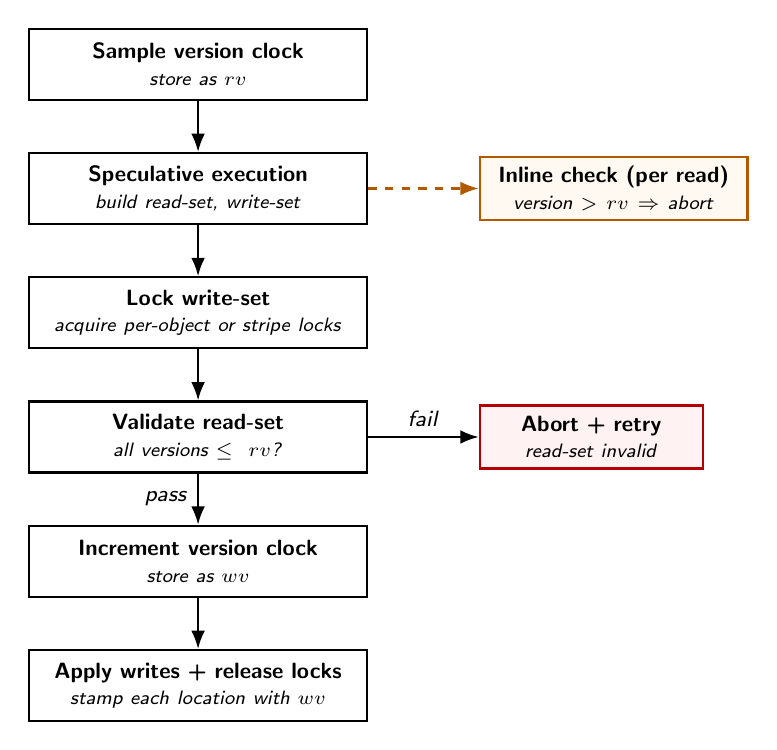
\begin{tikzpicture}[
    node distance = 0.65cm and 1.4cm,
    font = \sffamily\footnotesize,
    process/.style = {rectangle, minimum width=4.3cm, text width=3.9cm,
        minimum height=0.9cm, text centered, draw=black, thick,
        fill=white, align=center},
    abort/.style = {rectangle, minimum width=2.8cm, text width=2.6cm,
        minimum height=0.8cm, text centered, draw=red!70!black, thick,
        fill=red!5, align=center},
    inline/.style = {rectangle, minimum width=3.4cm, text width=3.0cm,
        minimum height=0.8cm, text centered, draw=orange!70!black, thick,
        fill=orange!5, align=center},
    arrow/.style = {thick, -{Latex[scale=1.0]}},
    darrow/.style = {thick, dashed, draw=orange!70!black, -{Latex[scale=1.0]}}
    ]
    \node (s1) [process] {\textbf{Sample version clock} \\
      \textit{\scriptsize store as $rv$}};
    \node (s2) [process, below=of s1] {\textbf{Speculative execution} \\
      \textit{\scriptsize build read-set, write-set}};
    \node (s3) [process, below=of s2] {\textbf{Lock write-set} \\
      \textit{\scriptsize acquire per-object or stripe locks}};
    \node (s4) [process, below=of s3] {\textbf{Validate read-set} \\
      \textit{\scriptsize all versions $\leq rv$?}};
    \node (s5) [process, below=of s4] {\textbf{Increment version clock} \\
      \textit{\scriptsize store as $wv$}};
    \node (s6) [process, below=of s5] {\textbf{Apply writes + release locks} \\
      \textit{\scriptsize stamp each location with $wv$}};

    \node (chk) [inline, right=of s2] {\textbf{Inline check (per read)} \\
      \textit{\scriptsize version $> rv \Rightarrow$ abort}};
    \node (ab1) [abort, right=of s4]  {\textbf{Abort + retry} \\
      \textit{\scriptsize read-set invalid}};

    \draw [arrow]  (s1) -- (s2);
    \draw [arrow]  (s2) -- (s3);
    \draw [arrow]  (s3) -- (s4);
    \draw [arrow]  (s4) -- node[left]{\textit{pass}} (s5);
    \draw [arrow]  (s5) -- (s6);
    \draw [darrow] (s2) -- (chk);
    \draw [arrow]  (s4) -- node[above]{\textit{fail}} (ab1);
  \end{tikzpicture}
  \caption{TL2 write transaction protocol.}
  \label{fig:tl2-write}
\end{figure}

TL2's separation of read-set and write-set, together with its global
version clock, provides the foundation for versioned data. While
TL2 itself keeps only the most recent version of each item, the
addition of version history would produce a design aligned with
MVCC. The design decisions and extensions adopted in this thesis are
discussed in Chapter~\ref{ch:implementation}.

\subsubsection{Synchronization Anomalies in STM}

Parri~\cite{parriTmIntro} presents a taxonomy of synchronization anomalies in
Software Transactional Memory. Because our STM system is based on optimistic MVCC,
dirty reads are excluded by design.
Two anomalies from Parri's taxonomy remain relevant:

\begin{itemize}
  \item \textbf{Non-Repeatable Read}: a transaction reads the same
        location twice and observes different values.
  \item \textbf{Intermediate Lost Update}: concurrent transactions modify
        overlapping locations and one update is silently overwritten.
\end{itemize}

In our system, non-repeatable reads are addressed
through Multi-Version Concurrency Control (MVCC) and read-set validation,
while intermediate lost updates are prevented through ownership-based conflict
resolution. These mechanisms are discussed further in
Sections~\ref{sec:reading} and~\ref{sec:conflict-resolution}.

\section{Existing Clojure STM Approaches and Limitations}

Clojure's STM exposes a concise API built around \texttt{dosync}, with
a function body, in which reads and writes to \texttt{Refs} are
executed atomically~\cite{clojureRefs}. The implementation is within
the \texttt{LockingTransaction} class.
Table~\ref{tab:clojure-stm} summarizes the key internal components of
\texttt{LockingTransaction} and \texttt{Ref}.

\begin{table}[htbp]
  \centering
  \small
  \begin{tabular}{lll}
    \toprule
    \textbf{Component} & \textbf{Field}      & \textbf{Role}                                     \\
    \midrule
    \multirow{5}{*}{\texttt{LockingTransaction}}
                       & \texttt{startPoint} & Globally unique transaction identifier            \\
                       & \texttt{readPoint}  & Snapshot point for MVCC reads                     \\
                       & \texttt{vals}       & In-transaction buffered write values              \\
                       & \texttt{sets}       & Refs modified via \texttt{alter}/\texttt{ref-set} \\
                       & \texttt{status}     & \texttt{RUNNING}, \texttt{COMMITTING},
    \texttt{COMMITTED}, \texttt{RETRY}, \texttt{KILLED}                                          \\
    \midrule
    \multirow{3}{*}{\texttt{Ref}}
                       & \texttt{tvals}      & Doubly linked history of committed values         \\
                       & \texttt{maxHistory} & Upper bound on retained versions                  \\
                       & \texttt{tinfo}      & Reference to owning transaction's \texttt{Info}   \\
    \bottomrule
  \end{tabular}
  \caption{Key internal fields of Clojure's STM implementation~\cite{jensen2016}.}
  \label{tab:clojure-stm}
\end{table}

A read inside a transaction calls \texttt{doGet}, which acquires a read lock
on the \texttt{Ref} and traverses \texttt{tvals} backwards to find the latest
committed value whose \texttt{point} does not exceed
\texttt{readPoint}~\cite{jensen2016}. If no such value exists, a fault counter
is incremented and the transaction retries, triggering an expansion of the
\texttt{Ref}'s history on the next attempt. A write calls \texttt{doSet},
which acquires a write lock on the \texttt{Ref}, adds it to \texttt{sets}, and
buffers the new value in \texttt{vals} without modifying shared memory until
commit~\cite{jensen2016}.

However, in contrast to its otherwise comprehensive STM design, transactions do
not support side-effects because they may be retried multiple times before
committing. Any side-effect performed within a transaction would therefore be
repeated on each retry.

\citeauthor{jensen2016}~\cite{jensen2016} addressed this by forking the
Clojure runtime and extending \texttt{LockingTransaction}, introducing
hooks such as \texttt{on-commit} and \texttt{after-commit}. While
effective, this approach couples the extension tightly to the runtime.

Rather than modifying \texttt{LockingTransaction}, we implement side-effect
support within our STM system at the language level. This avoids dependence
on a particular Clojure version while providing commit and rollback semantics.

Furthermore, Section~\ref{subsec:opacity-proof} shows that the resulting
system satisfies opacity~\cite{guerraoui2007}, providing formal correctness
guarantees for all transactions, including those that are aborted.
\chapter{Formal Model}
\label{ch:formal-model}

\textbf{Reader's Guide:} This chapter formalizes the concurrency control and
liveness properties of the proposed Software Transactional Memory (STM) system,
establishing the theoretical correctness on how the system handles opacity and global progress. The corresponding implementation is covered in
Chapter~\ref{ch:implementation}.

\section{Preliminaries}

To formally define the system, we abstract the state into two core
ideas: a timeline of global progress and the individual versioned variables.

Let $\mathcal{W}$ be the totally ordered set of \emph{write points}, where each
$w \in \mathcal{W}$ is a positive integer corresponding to a snapshot of the
global version clock. Let $\mathcal{R}$ be the set of \emph{transactional
references}, where each $r \in \mathcal{R}$ maintains a fixed
history of versioned values indexed by write points. Let $\mathcal{V}$ be the
set of all reference values.

Each reference $r \in \mathcal{R}$ is associated with a partial function
$\mathit{hist}(r) : \mathcal{W} \rightharpoonup \mathcal{V}$ that maps a write point to
the value committed at that point. For a transaction with read point $w_r$, the visible
value of $r$ is defined as:
\[
  \mathit{snap}(r,\, w_r)
    = \mathit{hist}(r)(w')
    \quad \text{where } w' = \max\bigl\{\, w \in \mathcal{W}
        \mid w \leq w_r,\; w \in \operatorname{dom}(\mathit{hist}(r)) \,\bigr\}
\]
That is, $\mathit{snap}$ returns the value committed at the latest write point that
(i)~does not exceed $w_r$ and (ii)~is in the domain of $\mathit{hist}(r)$, i.e.\ some
transaction actually wrote $r$ at that point.

\section{Transactions and Histories}

\begin{definition}[Transaction]
A transaction $T$ is a tuple $T = \langle\, id,\; w_r,\; RS,\; WS,\; \sigma
\,\rangle$ where:
\begin{itemize}
  \item $id \in \mathbb{N}$ is a unique monotonically increasing transaction
        identifier.
  \item $w_r \in \mathcal{W}$ is the \emph{read point}, the value of the
        global version clock at the time $T$ was created.
  \item $RS : \mathcal{R} \rightharpoonup \mathcal{W} \times \mathcal{V}$ is
        the \emph{read set}, mapping each reference read during $T$ to a tuple
        $e = (w, v)$ containing the write point and value observed.
  \item $WS : \mathcal{R} \rightharpoonup \mathcal{V}$ is the \emph{write set},
        mapping each reference to its speculative value.
  \item $\sigma \in \{\textsc{Active},\, \textsc{Aborted},\,
        \textsc{Committed}\}$ is the transaction status.
\end{itemize}
\end{definition}

\begin{definition}[History and Concurrency~{\cite{guerraoui2007,bushkov2012}}]
A \emph{history} $H$ of the system is a sequence of invocation and response
events produced by concurrent transactions. $H$ is \emph{well-formed} if for
every transaction $T$ in $H$, the events of $T$ form a sequence of alternating
invocations and responses.
\end{definition}

We consider only well-formed histories throughout. Following Bushkov et
al.~\cite{bushkov2012}, transaction $T$ is \emph{committed} if its last event
is a commit event and \emph{aborted} if its last event is an abort event.

\section{Operations}

Each transaction $T$ supports the following operations on references:

\paragraph{Read.} $\text{deref}(r)$ returns:
\[
  \text{deref}(r) =
  \begin{cases}
    WS[r]                  & \text{if } r \in \text{dom}(WS) \\
    RS[r].\mathit{value}   & \text{if } r \in \text{dom}(RS) \\
    \text{snap}(r,\; w_r)  & \text{otherwise}
  \end{cases}
\]

\paragraph{Write.}
$\text{ref-set}(r, v)$ requires $T$ to acquire ownership of $r$.
Let $\text{owner}(r) \in \mathbb{N} \cup \{ \bot \}$ denote the ID of the
transaction currently owning the speculative write for $r$.
Ownership is resolved as:
\[
\text{acquire}(T, r) =
\begin{cases}
    \text{True} & \text{if } \text{owner}(r) = \bot \lor \text{owner}(r) = T.id \\
    \text{True}, \sigma_{T'} \gets \textsc{Aborted} & \text{if } \text{owner}(r) = T'.id \land T'.id < T.id \\
    \text{Abort} & \text{if } \text{owner}(r) = T'.id \land T'.id > T.id
\end{cases}
\]
On success, $WS[r] \gets v$.

\section{Execution}

An \emph{execution} of transaction $T$ over function $f$ produces an outcome:
\[
  \text{execute}(T, f) =
  \begin{cases}
    \textsc{Ok}(v)
      & \text{if } f \text{ completes and } T \text{ commits successfully} \\
    \textsc{Abort}
      & \text{if an } \textsc{Aborted} \text{ signal is raised during } f \text{ or commit} \\
    \textsc{Exception}(e)
      & \text{if any other exception } e \text{ is raised}
  \end{cases}
\]

The transaction retry loop behaves as follows:
\[
\text{run-tx}(f, T) =
\begin{cases}
v
  & \text{if } \text{execute}(T,f)=\textsc{Ok}(v) \\[6pt]

\text{run-tx}(f, T')
  & \text{if } \text{execute}(T,f)=\textsc{Abort} \;\land\; T'=\text{next-tx}(T) \\[6pt]

\text{raise}(e)
  & \text{if } \text{execute}(T,f)=\textsc{Exception}(e)
\end{cases}
\]

where $\text{next-tx}(T)$ is a retry transition producing a new transaction with an incremented id, subject to retry limits.

\section{Commit Protocol}

A transaction $T$ with a non-empty write set ($\mathrm{dom}(WS) \neq \emptyset$) commits under a global commit lock. Upon entering the commit phase, the system checks $\sigma_T$. If $\sigma_T = \textsc{Aborted}$, the transaction is aborted and the commit is canceled.

If $T$ is still active, its read-set is validated against reference modifications by:
\[
\text{valid}(T) \triangleq \forall (r, e) \in RS:\;
\text{write-point}(r) \leq \text{write-point}(e)
\]

If $\text{valid}(T)$ does not hold, the transaction is aborted.

If validation succeeds, a new write point $w_c$ is allocated atomically. The transaction applies its writes to the global state and releases ownership of each written reference:
\[
    \text{owner}(r) \gets \bot \quad \forall\, r \in \mathrm{dom}(WS)
\]

Read-only transactions ($\mathrm{dom}(WS) = \emptyset$) skip the commit lock entirely, as their snapshot consistency is guaranteed by versioned reads.

\section{Safety: Opacity}

The correctness criterion of the proposed system is \emph{opacity}.
Intuitively, opacity guarantees that every transaction observes a logically consistent timeline, preventing crashes from unexpected states. Guerraoui and Kapalka~\cite{guerraoui2007} define opacity
through three requirements:
\begin{enumerate}
    \item \textbf{Atomicity:} Operations of committed transactions must appear
          to execute at a single indivisible point in time.
    \item \textbf{Isolation:} Operations of aborted transactions must never be
          visible to other transactions.
    \item \textbf{Consistency:} Every transaction must always observe a
          consistent system state, regardless of its final status.
\end{enumerate}

A \emph{completion} of a history $H$ is obtained by either appending a commit event or an
abort event to each transaction that has no final event in $H$, or by removing it
entirely. $\mathit{Complete}(H)$ denotes the set of all such completions~\cite{guerraoui2007}.

\begin{definition}[Opacity~{\cite{guerraoui2007}}]
A history $H$ is \emph{opaque} if there exists a sequential history $S$
equivalent to some history in $\text{Complete}(H)$, such that $S$ preserves
the real-time order of $H$ and every transaction $T_i \in S$ is \emph{legal}
in $S$.
\end{definition}

\begin{definition}[Legality~{\cite{guerraoui2007}}]
A transaction $T_j$ is \emph{legal} in a sequential history $S$ if, for every
reference $r$ read by $T_j$, the value observed is the value written by the
most recent committed transaction that wrote $r$ before $T_j$ in $S$, or the
initial value of $r$ if no such transaction exists.
\end{definition}

The key distinction from strict serializability is that opacity requires
legality for \emph{every} transaction in $S$, including aborted and live ones.
The proposed system guarantees opacity through two mechanisms:

\paragraph{Immutable Snapshots via $w_r$.}
Every transaction reads exclusively from the snapshot determined by its read
point $w_r$ via the $\text{snap}(r, w_r)$ function. Because these snapshots
are composed only of values from previously committed transactions, $T$ is
guaranteed to observe a state that was consistent at $w_r$.

\paragraph{Termination of Zombie Transactions.}
A status check before every critical operation ensures that no transaction
continues execution after its ownership has been stolen. This prevents zombie
transactions, those logically aborted but still physically executing,
from observing inconsistent states produced by concurrent writes after $w_r$.

Together, these properties ensure that every transaction observes only states
that could have arisen in a valid serial execution, satisfying opacity as
defined in~\cite{guerraoui2007}.

\begin{figure}[ht]
\centering
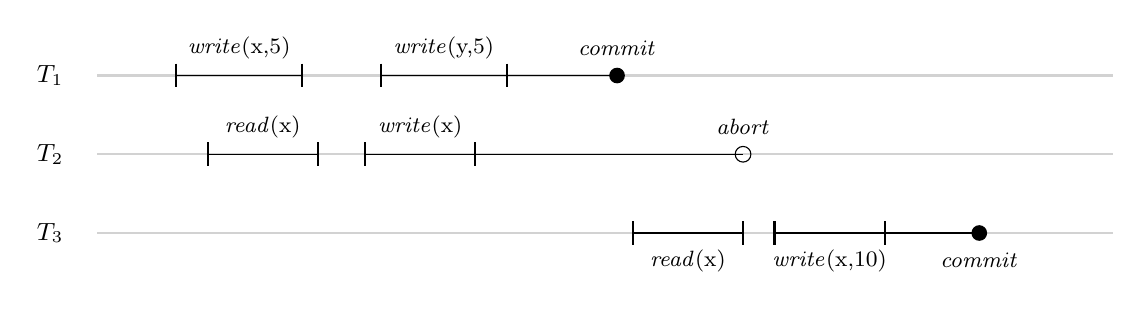
\begin{tikzpicture}[
  tx/.style={font=\small},
  op/.style={font=\footnotesize},
  line/.style={gray!35, thick},
  tick/.style={thick},
  commit/.style={circle, fill=black, inner sep=2pt},
  abort/.style={circle, draw, inner sep=2pt}
]
\node[tx] at (0,0)   {$T_1$};
\node[tx] at (0,-1)  {$T_2$};
\node[tx] at (0,-2)  {$T_3$};

\draw[line] (0.6,0) -- (13.5,0);
\draw[line] (0.6,-1) -- (13.5,-1);
\draw[line] (0.6,-2) -- (13.5,-2);

\draw (1.6,0) -- (3.2,0);
\draw[tick] (1.6,0.15)--(1.6,-0.15);
\draw[tick] (3.2,0.15)--(3.2,-0.15);
\node[op] at (2.4,0.35) {\textit{write}(x,5)};
\draw (4.2,0) -- (5.8,0);
\draw[tick] (4.2,0.15)--(4.2,-0.15);
\draw[tick] (5.8,0.15)--(5.8,-0.15);
\node[op] at (5.0,0.35) {\textit{write}(y,5)};
\draw (5.8,0) -- (7.2,0);
\node[commit] at (7.2,0) {};
\node[op] at (7.2,0.35) {\textit{commit}};

\draw (2.0,-1) -- (3.4,-1);
\draw[tick] (2.0,-0.85)--(2.0,-1.15);
\draw[tick] (3.4,-0.85)--(3.4,-1.15);
\node[op] at (2.7,-0.65) {\textit{read}(x)};
\draw (4.0,-1) -- (5.4,-1);
\draw[tick] (4.0,-0.85)--(4.0,-1.15);
\draw[tick] (5.4,-0.85)--(5.4,-1.15);
\node[op] at (4.7,-0.65) {\textit{write}(x)};
\draw (5.4,-1) -- (8.8,-1);
\node[abort] at (8.8,-1) {};
\node[op] at (8.8,-0.65) {\textit{abort}};

\draw (7.4,-2) -- (8.8,-2);
\draw[tick] (7.4,-1.85)--(7.4,-2.15);
\draw[tick] (8.8,-1.85)--(8.8,-2.15);
\node[op] at (8.1,-2.35) {\textit{read}(x)};
\draw (9.2,-2) -- (10.6,-2);
\draw[tick] (9.2,-1.85)--(9.2,-2.15);
\draw[tick] (10.6,-1.85)--(10.6,-2.15);
\node[op] at (9.9,-2.35) {\textit{write}(x,10)};
\draw (10.6,-2) -- (11.8,-2);
\node[commit] at (11.8,-2) {};
\node[op] at (11.8,-2.35) {\textit{commit}};
\end{tikzpicture}
\caption{An opaque history: $T_2$ is aborted but still observes a consistent
snapshot, satisfying the opacity requirement of~\cite{guerraoui2007}.}
\end{figure}

\section{Liveness: Impossibility of Local Progress and the Adopted Guarantee}

While safety ensures the system never returns an incorrect result, liveness
ensures the system makes forward progress under contention. A system that aborts
every transaction trivially satisfies opacity but makes no useful progress.
Formalising what progress a correct STM \emph{can} guarantee requires care, and
the theoretical bounds established by Bushkov and Guerraoui~\cite{bushkov2012}
directly shape the guarantees claimed here.

\paragraph{Starvation under adversarial scheduling.}
The impossibility of local progress manifests as \emph{starvation}. A
transaction $T_1$ that reads a reference $r$ may be indefinitely denied if a
succession of transactions $T_2, T_3, \ldots$ each write $r$ and commit before
$T_1$ can do so. Each such commit advances the write point of $r$ beyond $T_1$'s
read point, causing read-set validation to fail and forcing another retry. Under
adversarial scheduling this cycle repeats without bound. The proposed system does
not eliminate this possibility; doing so would contradict Theorem~1
of~\cite{bushkov2012}, since any mechanism guaranteeing $T_1$'s eventual commit
would require blocking concurrent writers, which is incompatible with opacity.

\begin{figure}[ht]
\centering
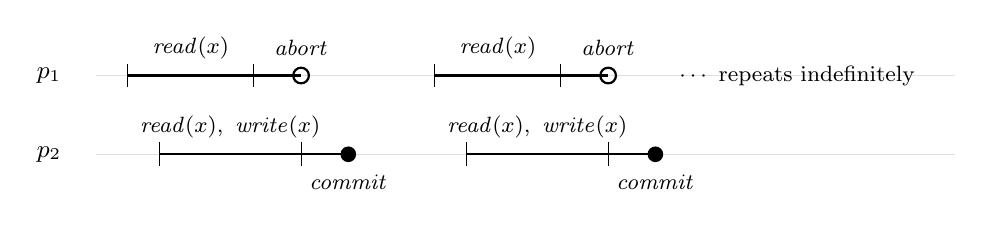
\begin{tikzpicture}[
  tx/.style={font=\small},
  op/.style={font=\footnotesize},
  tline/.style={thick},
  commit/.style={circle, fill=black, inner sep=2pt},
  abort/.style={circle, draw, thick, inner sep=2pt},
]
\node[tx] at (0, 0)  {$p_1$};
\node[tx] at (0, -1) {$p_2$};
\draw[gray!25] (0.6, 0) -- (11.5, 0);
\draw[gray!25] (0.6, -1) -- (11.5, -1);

\draw[tline] (1.0, 0) -- (2.6, 0);
\draw (1.0,0.15)--(1.0,-0.15); \draw (2.6,0.15)--(2.6,-0.15);
\node[op] at (1.8,0.35) {$\mathit{read}(x)$};
\draw[tline] (1.4, -1) -- (3.2, -1);
\draw (1.4,-0.85)--(1.4,-1.15); \draw (3.2,-0.85)--(3.2,-1.15);
\node[op] at (2.3,-0.65) {$\mathit{read}(x),\ \mathit{write}(x)$};
\draw[tline] (3.2,-1) -- (3.8,-1);
\node[commit] at (3.8,-1) {};
\node[op] at (3.8,-1.35) {\textit{commit}};
\draw[tline] (2.6,0) -- (3.2,0);
\node[abort] at (3.2,0) {};
\node[op] at (3.2,0.35) {\textit{abort}};

\draw[tline] (4.9, 0) -- (6.5, 0);
\draw (4.9,0.15)--(4.9,-0.15); \draw (6.5,0.15)--(6.5,-0.15);
\node[op] at (5.7,0.35) {$\mathit{read}(x)$};
\draw[tline] (5.3,-1) -- (7.1,-1);
\draw (5.3,-0.85)--(5.3,-1.15); \draw (7.1,-0.85)--(7.1,-1.15);
\node[op] at (6.2,-0.65) {$\mathit{read}(x),\ \mathit{write}(x)$};
\draw[tline] (7.1,-1) -- (7.7,-1);
\node[commit] at (7.7,-1) {};
\node[op] at (7.7,-1.35) {\textit{commit}};
\draw[tline] (6.5,0) -- (7.1,0);
\node[abort] at (7.1,0) {};
\node[op] at (7.1,0.35) {\textit{abort}};

\node[op] at (9.5, 0) {$\cdots$ repeats indefinitely};
\end{tikzpicture}
\caption{Starvation scenario: $p_2$ repeatedly commits before $p_1$, forcing
$p_1$ to abort forever.}
\end{figure}

\paragraph{Parasitic transactions.}
Bushkov et al.~\cite{bushkov2012} define a \emph{parasitic} process as one that
executes transactional operations indefinitely without ever invoking a commit
request. Such a process loops without committing but is repeatedly displaced by
newer transactions via ownership stealing, ensuring it never prevents progress
while its speculative state never reaches the committed history of any reference.

\begin{figure}[ht]
\centering
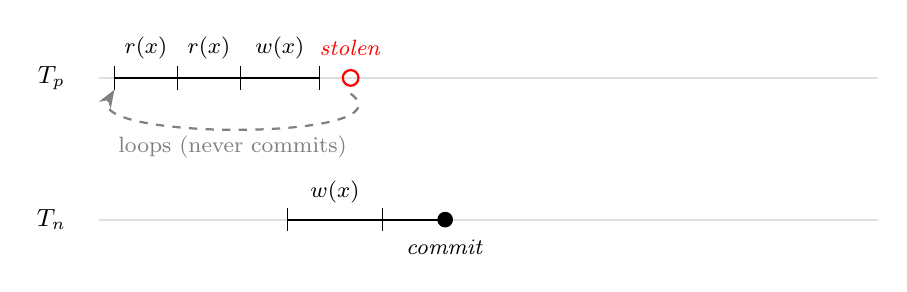
\begin{tikzpicture}[
  tx/.style={font=\small},
  op/.style={font=\footnotesize},
  line/.style={gray!25, thick},
  tline/.style={thick},
  commit/.style={circle, fill=black, inner sep=2pt},
  stolen/.style={circle, draw=red, thick, inner sep=2pt},
]
\node[tx] at (0, 0)    {$T_p$};
\node[tx] at (0, -1.8) {$T_n$};

\draw[line] (0.6, 0)    -- (10.5, 0);
\draw[line] (0.6, -1.8) -- (10.5, -1.8);

\draw[tline] (0.8,0) -- (1.6,0);
\draw (0.8,0.15)--(0.8,-0.15);
\draw (1.6,0.15)--(1.6,-0.15);
\node[op] at (1.2,0.38) {$r(x)$};

\draw[tline] (1.6,0) -- (2.4,0);
\draw (2.4,0.15)--(2.4,-0.15);
\node[op] at (2.0,0.38) {$r(x)$};

\draw[tline] (2.4,0) -- (3.4,0);
\draw (3.4,0.15)--(3.4,-0.15);
\node[op] at (2.9,0.38) {$w(x)$};

\node[stolen] at (3.8,0) {};
\node[op,red] at (3.8,0.38) {\textit{stolen}};

\draw[-{Stealth}, thick, dashed, gray]
  (3.8,-0.2) .. controls (4.6,-0.8) and (0.4,-0.8) .. (0.8,-0.15);
\node[op,gray] at (2.3,-0.88) {loops (never commits)};

\draw[tline] (3.0,-1.8) -- (4.2,-1.8);
\draw (3.0,-1.65)--(3.0,-1.95);
\draw (4.2,-1.65)--(4.2,-1.95);
\node[op] at (3.6,-1.45) {$w(x)$};
\draw[tline] (4.2,-1.8) -- (5.0,-1.8);
\node[commit] at (5.0,-1.8) {};
\node[op] at (5.0,-2.15) {\textit{commit}};
\end{tikzpicture}
\caption{A parasitic transaction $T_p$ loops indefinitely. A newer transaction
$T_n$ steals ownership (marked \textcolor{red}{\textit{stolen}}), aborting
$T_p$ and committing successfully. $T_p$ loops back and never reaches a commit,
but never blocks $T_n$ either.}
\end{figure}

\paragraph{Executions and outcomes.}
A single transaction attempt returns one of three outcomes:
$\textsc{Ok}(v)$ if the transaction committed successfully;
$\textsc{Abort}$ if the transaction was invalidated by a failed read-set check
or by ownership being stolen; or $\textsc{Exception}(e)$ if an unexpected error
propagated. The retry loop retries on $\textsc{Abort}$ and re-throws on
$\textsc{Exception}(e)$. If the retry count reaches a fixed maximum, the system
throws unconditionally rather than retrying indefinitely.

A \emph{history} $H$ of the system is the sequence of outcome events produced
by all threads over an execution. For a thread $p_k$ we write $H|_{p_k}$ for
the projection of $H$ onto the outcomes of that thread.

\paragraph{Process classifications.}
Following Bushkov and Guerraoui~\cite{bushkov2012}, threads are partitioned into
classes according to their observable behaviour in a history.

\begin{definition}[Correct Process~{\cite{bushkov2012}}]
A thread $p_k$ is \emph{correct} in $H$ if $H|_{p_k}$ contains infinitely many
$\textsc{Ok}(v)$ or $\textsc{Abort}$ outcomes: that is, $p_k$ persists
indefinitely without exiting via $\textsc{Exception}(e)$.
\end{definition}

\begin{definition}[Crashed Process~{\cite{bushkov2012}}]
A thread $p_k$ is \emph{crashed} in $H$ if $H|_{p_k}$ is finite. The history
is augmented with a crash event $\mathit{crash}^k$ immediately after the last
outcome of $p_k$.
\end{definition}

\begin{definition}[Parasitic Process~{\cite{bushkov2012}}]
A thread $p_k$ is \emph{parasitic} in $H$ if $H|_{p_k}$ contains infinitely
many outcomes but only $\textsc{Abort}$ outcomes from some point onward, with no
intervening $\textsc{Ok}(v)$, due to the thread never reaching the commit phase.
\end{definition}

\paragraph{Progress.}
A correct thread $p_k$ \emph{makes progress} in $H$ if $H|_{p_k}$ contains
infinitely many $\textsc{Ok}(v)$ outcomes. A thread producing only
$\textsc{Abort}$ outcomes indefinitely is \emph{starved}.

\paragraph{Local progress and its impossibility.}

\begin{definition}[Local Progress~{\cite{bushkov2012}}]
A history $H$ ensures \emph{local progress} if every correct thread makes
progress:
\[
  H \text{ ensures local progress} \;\iff\;
  \forall\, p_k \in \mathit{Correct}(H) :\;
  |\{\,\textsc{Ok}(v) \in H|_{p_k}\}| = \infty
\]
\end{definition}

Theorem~1 of Bushkov and Guerraoui~\cite{bushkov2012} establishes that no TM
implementation can ensure both opacity and local progress in a fault-prone
system. The proposed system does not claim local progress; doing so would
require blocking concurrent writers, which is incompatible with opacity.

\paragraph{Global progress as the adopted guarantee.}

\begin{definition}[Global Progress~{\cite{bushkov2012}}]
A history $H$ ensures \emph{global progress} if at least one correct thread
makes progress:
\[
  H \text{ ensures global progress} \;\iff\;
  \exists\, p_k \in \mathit{Correct}(H) :\;
  |\{\,\textsc{Ok}(v) \in H|_{p_k}\}| = \infty
\]
\end{definition}

Global progress is strictly weaker than local progress and is compatible with
opacity~\cite{bushkov2012}.

\begin{theorem}[Deadlock Freedom and Global Progress]
Let $\prec$ be the total strict ordering on transactions defined by
$T_i \prec T_j \iff T_i.id < T_j.id$. The ownership-resolution policy
guarantees that the implementation is deadlock-free and ensures global
progress in the sense of~\cite{bushkov2012}.
\end{theorem}

\begin{proof}
Since $id$ is assigned from a global monotonically increasing atomic counter,
$\prec$ forms a strict total order over all created transactions. Ownership of
a reference $r$ is granted to $T_j$ over $T_i$ if and only if $T_i \prec T_j$.
Because a transaction can only be preempted by one strictly greater in $\prec$,
cyclic dependencies are impossible, establishing deadlock freedom.

In any non-empty set of competing transactions, there exists $T_{max}$ such that
$\forall T_i \neq T_{max}: T_i \prec T_{max}$. $T_{max}$ successfully acquires
all required ownerships without being aborted. It then enters the commit phase,
where read-set validation ensures its snapshot remains consistent. Thus in every
contention round at least one correct process is guaranteed to commit,
satisfying global progress.
\end{proof}

\paragraph{Termination under absence of contention.}
A transaction $T$ that encounters no conflicting concurrent writes commits on
its first attempt. The validation condition is trivially satisfied when no other
transaction has written to any ref in $RS$ since $w_r$.

\paragraph{Progress under contention via ownership stealing.}
When two transactions $T_i$ and $T_j$ compete for the same reference, the one
with the strictly greater identifier is granted ownership:
\[
  \text{owner}(r) \gets T_j.id \quad \text{if } T_j.id > T_i.id,\quad
  \sigma_{T_i} \gets \textsc{Aborted}
\]
This guarantees at least one winner per contention round. It is, however, the
same mechanism responsible for starvation: a transaction repeatedly preempted by
newer ones may never obtain ownership long enough to commit. This is precisely
the trade-off admitted by~\cite{bushkov2012}: global progress is achievable but
local progress is not.

\paragraph{Bounded backoff.}
When a transaction is aborted and retried, exponential backoff with jitter is applied
after the fourth retry. The delay grows with the retry count up to a fixed cap of
$32\,\text{ms}$, with $\pm 25\%$ random jitter to prevent the thundering-herd problem.
Because the cap is finite, worst-case per-retry latency is bounded regardless of
contention level. The precise formula is given in Section~\ref{sec:retry}.
\chapter{Implementation}
\label{ch:implementation}

The complete source code is publicly available at~\cite{chapidze2026opusdb}.

\section{Alignment with TL2}
This implementation follows the structure of Transactional Locking II
(TL2)~\cite{dice2006transactional}, but departs from the original in three
ways.

TL2 supports two lock-mapping policies: per-object (PO), where each reference
carries its own versioned lock, and per-stripe (PS), where each
reference hashes to a lock in a fixed array~\cite{dice2006transactional}.
Neither is used here. Ownership acquisition at write time instead goes
through a dedicated \texttt{java.lang.Object} monitor per reference, while
commit serialization is handled separately, by a single global commit lock.

TL2 discovers write conflicts at commit time; here they're caught earlier,
\emph{eagerly}, at the point of write, via \texttt{try-acquire!}, so a
losing transaction aborts on the spot rather than wasting work on a
transaction it's about to abort anyway.

TL2 also keeps only the most recently committed value of each reference.
This implementation adds \emph{Multi-Version Concurrency Control
  (MVCC)}~\cite{bernstein1983} on top, keeping a bounded version history
per reference so readers can find a consistent snapshot without
blocking writers (see Section~\ref{sec:mvcc-design}).

\section{Architecture Overview}
The \texttt{opusdb.atomic.stm} namespace defines four global data structures
and four constants that coordinate all transactional activity.

\begin{description}
  \item[\texttt{write-point}] An \texttt{AtomicLong} serving as the version
        clock, incremented atomically on every successful write-transaction
        commit to establish a total order over committed states.
  \item[\texttt{tx-counter}] A monotonically increasing \texttt{AtomicLong}
        that assigns unique transaction identifiers, whose ordering forms the
        basis of the ownership protocol.
  \item[\texttt{active-tx}] A \texttt{ConcurrentHashMap} mapping live
        transaction IDs to their transaction maps, used to locate and abort
        the owner of a conflicting reference.
  \item[\texttt{commit-lock}] A single global \texttt{Object} monitor that
        serializes read-set validation and write application across all write
        transactions.
\end{description}

Four constants tune the runtime behaviour:

\begin{description}
  \item[\texttt{max-history} (32)] Maximum size of a version history per
        reference; older entries are discarded on commit.
  \item[\texttt{max-retries} (96)] Maximum retries before throwing
        unconditionally. At roughly 2 seconds of cumulative delay, a
        still-failing transaction is assumed to be in livelock.
  \item[\texttt{base-sleep-ms} (1) and \texttt{max-sleep-ms} (32)] Bounds
        of the exponential backoff delay applied after the fourth retry,
        capped at 32\,ms to keep worst-case latency bounded.
\end{description}

The current transaction is bound to the thread-local variable \texttt{*tx*},
with \texttt{nil} indicating no active transaction context.

\section{Reference and Version History}

A transactional reference is created by \texttt{ref}, which packages the
initial value, version history, and ownership metadata into a single Clojure
\texttt{atom}:

\begin{listing}[H]
  \begin{minted}{clojure}
(defn ref [initial-val]
  (let [wp    (.get write-point)
        entry {:value initial-val :write-point wp}]
    (atom {:value       initial-val
           :write-point wp
           :history     [entry]
           :owner       nil
           :lock        (Object.)})))
\end{minted}
  \caption{Reference structure.}
  \label{lst:ref-structure}
\end{listing}

The \texttt{:history} vector stores committed versions as
\texttt{\{:value v :write-point w\}} entries. The \texttt{:lock} field is a
dedicated \texttt{Object} monitor; \texttt{try-acquire!} synchronizes on it
when competing transactions claim ownership of the same reference.

Version history is bounded by \texttt{max-history = 32}. When a commit would
push the count beyond this limit, \texttt{trim-history} drops the oldest
entry before appending the new one:

\begin{listing}[H]
  \begin{minted}{clojure}
(defn- trim-history [history]
  (if (> (count history) max-history)
    (vec (take-last max-history history))
    history))
\end{minted}
  \caption{History trimming.}
  \label{lst:trim-history}
\end{listing}

\section{Transaction Lifecycle}

\begin{figure}[H]
  \centering
  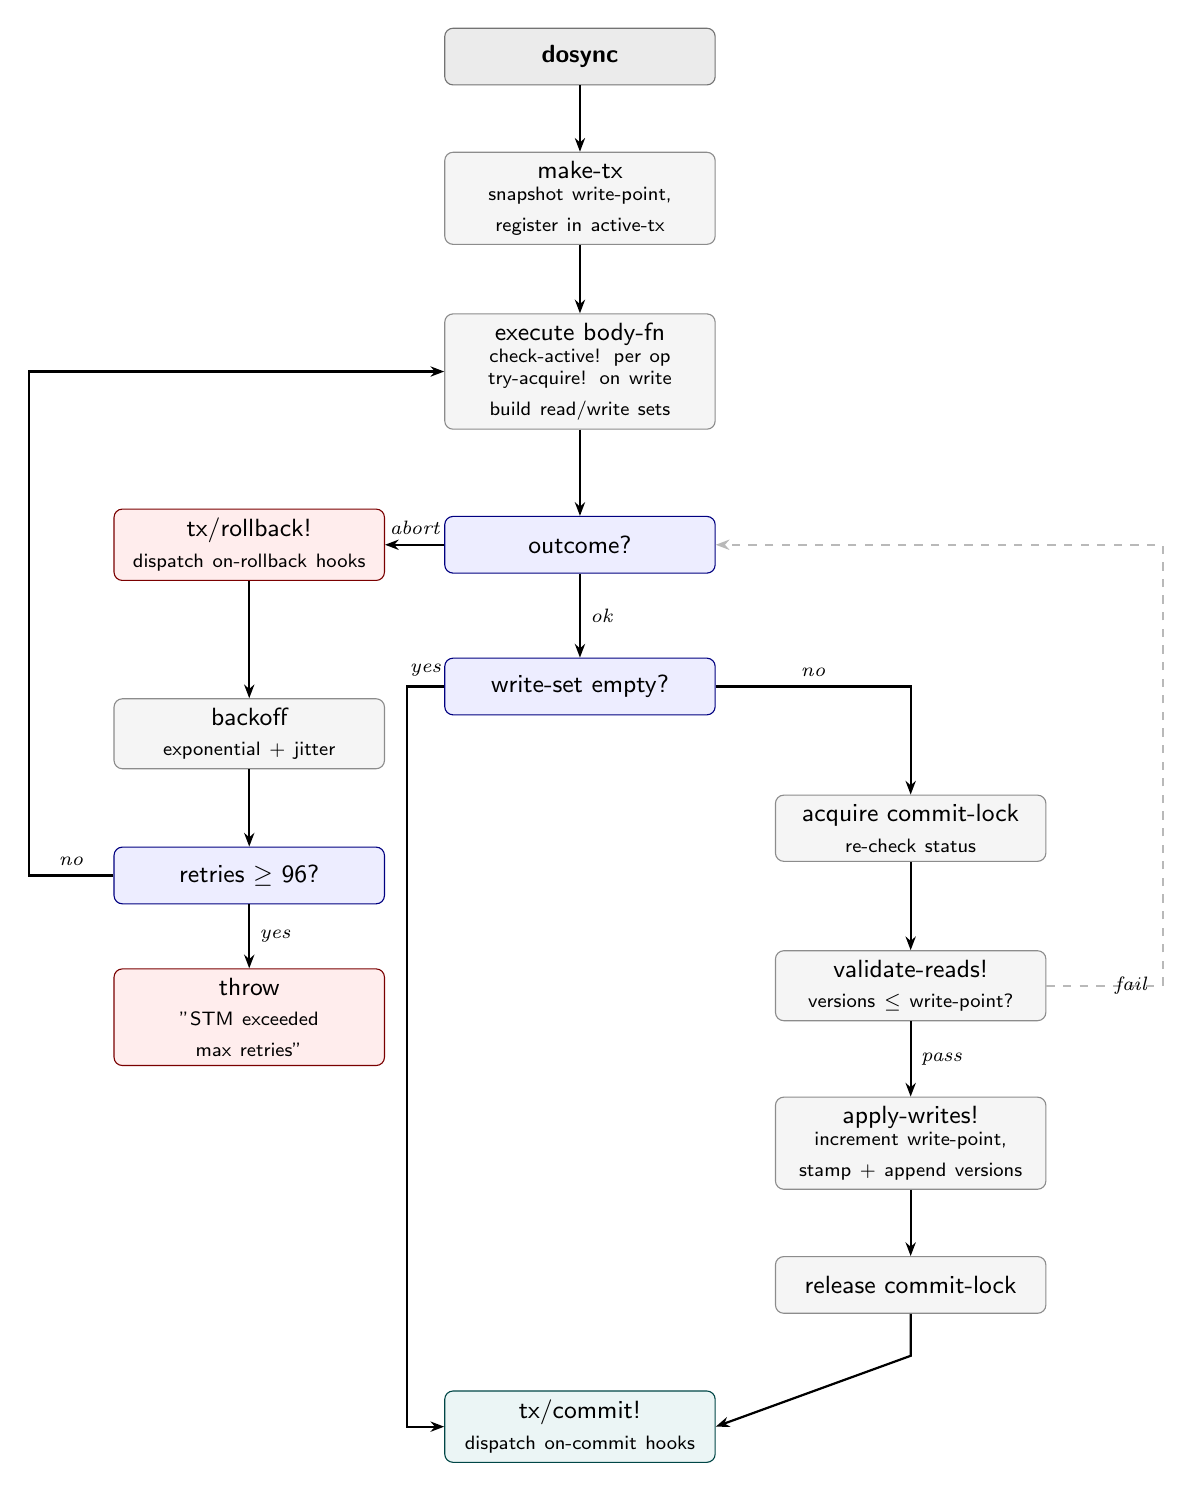
\begin{tikzpicture}[
    font=\sffamily\small,
    every node/.style={align=center},
    N/.style={
        rectangle, rounded corners=3pt,
        draw=black!45, fill=gray!8,
        minimum width=3.4cm, minimum height=0.72cm,
        text width=3.2cm},
    D/.style={N, draw=blue!50!black, fill=blue!7},
    OK/.style={N, draw=teal!55!black, fill=teal!8},
    AB/.style={N, draw=red!48!black,  fill=red!7},
    T/.style={N, draw=black!55, fill=gray!16,
        font=\sffamily\small\bfseries},
    a/.style={-{Stealth[scale=0.75]}, thick},
    d/.style={-{Stealth[scale=0.75]}, thick, dashed, draw=gray!55},
    ]
    \def\lx{-4.2}
    \def\cx{0}
    \def\rx{4.2}
    \def\loopx{-7.0}
    \def\routeR{7.4}
    \def\readonlyL{-2.2}

    \node[T]  (s)  at (\cx,   0.0) {dosync};
    \node[N]  (mt) at (\cx,  -1.8) {make-tx\\
    {\scriptsize snapshot write-point,\\register in active-tx}};
    \node[N]  (bf) at (\cx,  -4.0) {execute body-fn\\
    {\scriptsize check-active! per op\\
    try-acquire! on write\\
    build read/write sets}};
    \node[D]  (oc) at (\cx,  -6.2) {outcome?};
    \node[D]  (we) at (\cx,  -8.0) {write-set empty?};

    \node[N]  (al) at (\rx,  -9.8) {acquire commit-lock\\
    {\scriptsize re-check status}};
    \node[N]  (vr) at (\rx, -11.8) {validate-reads!\\
    {\scriptsize versions $\leq$ write-point?}};
    \node[N]  (aw) at (\rx, -13.8) {apply-writes!\\
    {\scriptsize increment write-point,\\stamp + append versions}};
    \node[N]  (rl) at (\rx, -15.6) {release commit-lock};
    \node[OK] (cm) at (\cx, -17.4) {tx/commit!\\
    {\scriptsize dispatch on-commit hooks}};

    \node[AB] (rb) at (\lx,  -6.2) {tx/rollback!\\
    {\scriptsize dispatch on-rollback hooks}};
    \node[N]  (bk) at (\lx,  -8.6) {backoff\\
    {\scriptsize exponential + jitter}};
    \node[D]  (mr) at (\lx, -10.4) {retries $\geq$ 96?};
    \node[AB] (th) at (\lx, -12.2) {throw\\
    {\scriptsize "STM exceeded max retries"}};

    \draw[a] (s)  -- (mt);
    \draw[a] (mt) -- (bf);
    \draw[a] (bf) -- (oc);
    \draw[a] (oc) -- node[right, font=\scriptsize\itshape]{ok} (we);

    \draw[a] (we.west)
    -- node[above, font=\scriptsize\itshape]{yes}
    (\readonlyL,-8.0)
    -- (\readonlyL,-17.4)
    -- (cm.west);

    \draw[a] (we.east)
    -- node[above, font=\scriptsize\itshape]{no}
    (\rx,-8.0)
    -- (al.north);
    \draw[a] (al) -- (vr);
    \draw[a] (vr) -- node[right, font=\scriptsize\itshape]{pass} (aw);
    \draw[a] (aw) -- (rl);
    \draw[a] (rl.south) -- (\rx,-16.5) -- (cm.east);

    \draw[d] (vr.east)
    -- node[right, font=\scriptsize\itshape]{fail}
    (\routeR,-11.8)
    -- (\routeR,-6.2)
    -- (oc.east);

    \draw[a] (oc.west)
    -- node[above, font=\scriptsize\itshape]{abort}
    (rb.east);
    \draw[a] (rb) -- (bk);
    \draw[a] (bk) -- (mr);
    \draw[a] (mr) -- node[right, font=\scriptsize\itshape]{yes} (th);

    \draw[a] (mr.west)
    -- node[above, font=\scriptsize\itshape]{no}
    (\loopx,-10.4)
    -- (\loopx,-4.0)
    -- (bf.west);

  \end{tikzpicture}
  \caption{Transaction execution flow. The speculative phase builds read/write
    sets, checking status and acquiring ownership on each write; on success
    the commit path validates read-set, applies writes under the commit lock
    (read-only transactions bypass the commit lock entirely), and dispatches
    commit hooks; on failure the abort path dispatches rollback hooks, backs off,
    and retries with a fresh snapshot.}
  \label{fig:tx-flow}
\end{figure}

The subsections below walk through each phase.

\subsection{Creation}

Each transaction is created by \texttt{make-tx}, which atomically increments
\texttt{tx-counter} to obtain a unique identifier, snapshots the current
\texttt{write-point} as the read point, initializes empty read and write sets,
and registers the transaction in \texttt{active-tx}:

\begin{listing}[H]
  \begin{minted}{clojure}
(defn- make-tx [retry-count]
  (let [id (.incrementAndGet tx-counter)
        tx {:id          id
            :read-point  (.get write-point)
            :read-set    (IdentityHashMap.)
            :write-set   (IdentityHashMap.)
            :retry-count retry-count
            :status      (volatile! ::active)}]
    (.put active-tx id tx)
    tx))
\end{minted}
  \caption{Transaction creation. The read point is snapshotted at creation
    time, defining the consistent view of memory this transaction will observe.}
  \label{lst:make-tx}
\end{listing}

Both the read-set and write-set use \texttt{IdentityHashMap}, which compares
keys by reference identity rather than value equality. This matters because
transactional references are \texttt{atom} objects: their identity stays
fixed for life, even as their contents change on every commit.

The read-set also caches the \texttt{:write-point} observed at read time
alongside the value. Since the reference's own \texttt{:write-point} field
gets overwritten by later commits, read-set validation would otherwise have
nothing left to compare against when checking for conflicts.

\subsection{Reading}
\label{sec:reading}

\texttt{deref} resolves a reference value through three ordered lookups:

\begin{listing}[H]
  \begin{minted}{clojure}
(defn deref [target-ref]
  (if-not *tx*
    (:value @target-ref)
    (let [tx        *tx*
          write-set (:write-set tx)
          read-set  (:read-set tx)]
      (check-active! tx)

      (cond
        (.containsKey write-set target-ref)
        (.get write-set target-ref)

        (.containsKey read-set target-ref)
        (:value (.get read-set target-ref))

        :else
        (let [snapshot (find-entry (:read-point tx)
                                   (:history @target-ref))]
          (when-not snapshot (abort))
          (.put read-set target-ref snapshot)
          (:value snapshot))))))
  \end{minted}
  \caption{Transactional read. The write-set is checked first for
    read-your-writes semantics; the read-set returns the previously cached
    snapshot; the version history is checked last.}
  \label{lst:deref}
\end{listing}

Checking the write-set first guarantees read-your-writes: a transaction
always sees whatever it has already buffered. After that comes the
read-set: if the reference was already read earlier in the same
transaction, its cached snapshot comes back directly. Only when neither set
has it does \texttt{find-entry} search the history, returning the latest
committed entry whose write point doesn't exceed the transaction's read
point. If the history has been trimmed past the point where such an entry
exists, the transaction aborts and retries with a fresh snapshot.

\subsection{Writing}

\texttt{ref-set} buffers a write into the transaction's write-set, but only
after acquiring ownership of the target reference via \texttt{try-acquire!}:

\begin{listing}[H]
  \begin{minted}{clojure}
(defn ref-set [target-ref new-val]
  (when-not *tx*
    (throw (IllegalStateException. "ref-set outside transaction")))
  (let [tx *tx*]
    (check-active! tx)
    (when-not (try-acquire! target-ref tx)
      (abort))
    (.put ^IdentityHashMap (:write-set tx) target-ref new-val)
    new-val))
\end{minted}
  \caption{Transactional write. Ownership must be acquired before buffering;
    failure to acquire triggers an immediate abort.}
  \label{lst:ref-set}
\end{listing}

\texttt{alter} is a thin convenience wrapper: it reads the current value and
hands it to a caller-supplied function before delegating to \texttt{ref-set}:

\begin{listing}[H]
  \begin{minted}{clojure}
(defn alter [target-ref f & args]
  (ref-set target-ref (apply f (deref target-ref) args)))
\end{minted}
  \caption{alter reads the current value and writes the result of applying
    \texttt{f}, reusing the ownership and buffering logic of \texttt{ref-set}.}
  \label{lst:alter}
\end{listing}

\subsection{Committing}

\texttt{commit!} finalizes a transaction. Read-only transactions, those
with an empty write-set, skip the global commit lock entirely and commit
right away, since the version history already guarantees their snapshot is
consistent. Write transactions don't get that shortcut: they enter the
commit lock, re-check their status (ownership theft can happen while
waiting), validate the read-set, and only then apply their writes:

\begin{listing}[H]
  \begin{minted}{clojure}
(defn- commit! [tx]
  (check-active! tx)
  (let [{:keys [id read-set write-set status]} tx]
    (when (seq write-set)
      (locking commit-lock
        (check-active! tx)
        (validate-reads! read-set)
        (apply-writes! write-set)))
    (vreset! status ::committed)
    (.remove active-tx id)
    (tx/commit! id)))
\end{minted}
  \caption{Commit protocol. Read-only transactions skip the commit lock;
    write transactions validate reads before applying writes.}
  \label{lst:commit}
\end{listing}

\texttt{apply-writes!} increments \texttt{write-point} exactly once and uses
that value to timestamp every write in the batch, which is what keeps all
writes from one commit atomic with respect to readers:

\begin{listing}[H]
  \begin{minted}{clojure}
(defn- apply-writes! [^IdentityHashMap write-set]
  (let [commit-point (.incrementAndGet write-point)]
    (doseq [[r new-val] write-set]
      (swap! r (fn [{:keys [history] :as state}]
                 (assoc state
                        :value       new-val
                        :write-point commit-point
                        :owner       nil
                        :history     (trim-history
                                      (conj history
                                            {:value       new-val
                                             :write-point commit-point}))))))))
\end{minted}
  \caption{Write application. A single increment of the global write point
    timestamps all writes in a commit atomically.}
  \label{lst:apply-writes}
\end{listing}

\subsection{Retry and Backoff}
\label{sec:retry}

When a transaction aborts, \texttt{next-tx} dispatches its rollback hooks,
removes it from \texttt{active-tx}, and hands back a fresh transaction with
an incremented retry count. The first four retries carry no sleep penalty at
at all, since short-lived conflicts that resolve quickly shouldn't have to pay for a
\texttt{Thread/sleep} call. Past the fourth retry, backoff kicks in, and if
\texttt{max-retries} $= 96$ is ever reached the system throws unconditionally,
on the assumption that this is most likely a livelock by that point.

For retry count $n > 4$, the sleep duration is:
\begin{equation}
  S = b(n)\!\left(1 + \tfrac{1}{4}X\right), \quad X \sim \mathcal{U}[-1,1]
\end{equation}
with bounds $S_{\min} = \tfrac{3}{4}b(n)$, $S_{\max} = \tfrac{5}{4}b(n)$,
and base delay:
\begin{equation}
  b(n) = \min\!\left(32,\; 2^{\min(n-4,\,6)}\right)\,\text{ms}
\end{equation}
giving $b(5) = 2\,\text{ms}$, $b(8) = 16\,\text{ms}$, and $b(n) = 32\,\text{ms}$
for all $n \geq 9$. The $\pm 25\%$ jitter exists to prevent the
thundering-herd problem\footnote{The thundering-herd problem occurs when multiple transactions
  abort simultaneously and retry at the same time, causing them to conflict again
  and repeat the cycle. Jitter breaks the symmetry by randomizing each
  transaction's retry delay.}, spreading retry attempts out over time; the
$32\,\text{ms}$ cap keeps worst-case per-retry latency bounded no matter how
severe the contention gets.

\begin{listing}[H]
  \begin{minted}{clojure}
(defn- next-tx [current]
  (tx/rollback! (:id current))
  (.remove active-tx (:id current))
  (let [retries (:retry-count current)]
    (when (>= retries max-retries)
      (throw (ex-info "STM exceeded max retries" {:retries retries})))
    (when (> retries 4)
      (let [base   (min max-sleep-ms
                        (bit-shift-left base-sleep-ms
                                        (min (- retries 4) 6)))
            jitter (long (* base 0.25
                            (- (* 2 (.nextDouble
                                      (ThreadLocalRandom/current)))
                               1)))]
        (Thread/sleep (max 0 (long (+ base jitter))))))
    (make-tx (inc retries))))
\end{minted}
  \caption{Retry with bounded exponential backoff. The four-retry period
    avoids sleep overhead for short-lived conflicts.}
  \label{lst:next-tx}
\end{listing}

\subsection{The dosync Macro}

\texttt{dosync} is a thin macro over \texttt{sync}, which checks whether a
transaction is already active on the current thread; if not, \texttt{run-tx}
starts a new transaction loop:

\begin{listing}[H]
  \begin{minted}{clojure}
(defn sync [body-fn]
  (if *tx*
    (body-fn)
    (run-tx body-fn)))

(defmacro dosync [& body]
  `(sync (fn* [] ~@body)))
\end{minted}
  \caption{\texttt{dosync} delegates to \texttt{sync}, which joins an existing
    transaction if one is active, or starts a new one via \texttt{run-tx}.}
  \label{lst:dosync}
\end{listing}

\paragraph{Nested transaction semantics.}
When \texttt{dosync} runs on a thread that already has a transaction bound
to \texttt{*tx*}, \texttt{sync} just invokes the body inside that existing
transaction rather than opening a new one, which is \emph{flat nesting}. The inner
call shares the outer transaction's read-set, write-set, and snapshot, so an
abort anywhere in the inner body propagates outward and the whole
transaction retries. Hooks registered inside the inner body get associated
with the outer transaction's identifier, so they still fire at the right
lifecycle boundary. This is exactly the composability property described in
Section~\ref{sec:intro}: \texttt{withdraw} and \texttt{deposit} each have
their own \texttt{dosync}, but called inside an enclosing \texttt{dosync}
they end up participating in a single atomic transaction.
Figure~\ref{fig:tx-flow} lays out the full execution flow.

\section{Conflict Resolution}
\label{sec:conflict-resolution}

Rather than waiting until commit time to detect conflicts, the system
resolves write conflicts the moment a transaction first touches a reference.
\texttt{try-acquire!} claims ownership under that reference's per-ref
monitor, following an ownership protocol that favours the younger
transaction: a transaction with a higher identifier preempts whoever holds
ownership currently, marking them aborted, which they'll notice on
their next \texttt{check-active!} call. An older transaction that loses the
contest aborts itself right away and retries. The \texttt{max-retries} bound
from Section~\ref{sec:retry} keeps a repeatedly preempted transaction from
spinning forever.

\begin{listing}[H]
  \begin{minted}{clojure}
(defn- try-acquire! [target-ref tx]
  (let [claimer-id (:id tx)
        lock       (:lock @target-ref)]
    (monitor-enter lock)
    (try
      (let [owner-id (:owner @target-ref)]
        (cond
          (nil? owner-id)
          (do (swap! target-ref assoc :owner claimer-id) true)
          (= owner-id claimer-id)
          true
          (> claimer-id owner-id)
          (do (when-some [owner-tx (.get active-tx owner-id)]
                (when (= @(:status owner-tx) ::active)
                  (vreset! (:status owner-tx) ::aborted)))
              (swap! target-ref assoc :owner claimer-id)
              true)
          :else false))
      (finally
        (monitor-exit lock)))))
\end{minted}
  \caption{Ownership acquisition. Younger transactions preempt the older
    owner, which aborts and retries.}
  \label{lst:try-acquire}
\end{listing}

The four \texttt{cond} branches cover every possible ownership state. An
unowned reference gets claimed immediately. A reference already owned by the
same transaction is just a no-op, which comes up when \texttt{ref-set} gets
called more than once on the same ref. If the current owner is older, the
claimer marks it \textsc{Aborted} in \texttt{active-tx} atomically and takes
over; if the current owner is younger, the claimer backs off instead,
returning \texttt{false} and aborting so the younger transaction has room to
finish.

The aborted owner finds out about its own invalidation the next time
\texttt{check-active!} runs, which happens before every critical operation,
and exits without committing any partial state.

\section{MVCC Design}
\label{sec:mvcc-design}

The system extends TL2 with multi-version concurrency
control~\cite{bernstein1983} by maintaining a bounded version history per
reference. Each history entry records a committed value and the write point
it was committed at. When a transaction commits at write point $w_c$, the
history of each written reference updates as:
\[
  \text{hist}_{\text{new}}(r) = \text{trim}_{32}\!\left(
  \text{hist}_{\text{old}}(r) \cup \bigl\{ (w_c,\; WS[r]) \bigr\}
  \right)
\]
where $\text{trim}_{32}$ drops the oldest entry if the count would exceed
\texttt{max-history}.

A transaction with read point $w_r$ retrieves the visible value of reference
$r$ via \texttt{find-entry}, which walks the history newest-to-oldest and
returns the first entry whose write point doesn't exceed $w_r$:

\begin{listing}[H]
  \begin{minted}{clojure}
(defn- find-entry [read-point history]
  (loop [i (dec (count history))]
    (when (>= i 0)
      (let [entry (nth history i)]
        (if (<= (:write-point entry) read-point)
          entry
          (recur (dec i)))))))
\end{minted}
  \caption{Version history scan. Newest-first traversal returns the latest
    version visible at the transaction's read point.}
  \label{lst:find-entry}
\end{listing}

In practice, this means readers and writers never block each other. A reader
at $w_r$ simply picks up a snapshot from before any concurrent writer's
commit, so neither side ever waits on the other. It's this property that
drives the strong scaling seen in the read-heavy benchmark of
Section~\ref{sec:read-write-heavy}: readers never touch the commit-lock
path at all.

If a transaction's read point falls below the oldest retained entry, no
valid snapshot exists, and the transaction aborts immediately and retries
with a fresh read point.

\section{Transactional Event System}

Side-effects are unsafe inside a transaction body, since that body may run
many times before a commit actually succeeds. Logging, sending a
notification, or writing to an external system on the first attempt would
fire again on every subsequent retry. The transactional event system in the
\texttt{opusdb.atomic.tx-hooks} namespace solves this by deferring handler
execution to a well-defined lifecycle boundary instead.

Two hooks are provided. \texttt{on-commit} schedules a handler to run
exactly once, after a successful commit. \texttt{on-rollback} schedules one
to run on each abort, before the next retry, which is useful for cleanup or
diagnostic logging:

\begin{listing}[H]
  \begin{minted}{clojure}
(defn on-commit [handler]
  (if *tx*
    (tx/on-commit (:id *tx*) handler)
    (throw (IllegalStateException. "on-commit outside transaction"))))

(defn on-rollback [handler]
  (if *tx*
    (tx/on-rollback (:id *tx*) handler)
    (throw (IllegalStateException. "on-rollback outside transaction"))))
\end{minted}
  \caption{Hook registration. Handlers are associated with a transaction ID
    and dispatched at the appropriate lifecycle event.}
  \label{lst:hook-registration}
\end{listing}

Storage underneath uses two \texttt{ConcurrentHashMap} instances, one for
commit handlers and one for rollback handlers, both indexed by transaction
ID:

\begin{listing}[H]
  \begin{minted}{clojure}
(def ^:private ^ConcurrentHashMap COMMIT_EVENTS   (ConcurrentHashMap.))
(def ^:private ^ConcurrentHashMap ROLLBACK_EVENTS (ConcurrentHashMap.))

(defn on-commit [id fun]
  (.compute COMMIT_EVENTS id
            (fn [_ fns] (conj (or fns []) fun))))

(defn on-rollback [id fun]
  (.compute ROLLBACK_EVENTS id
            (fn [_ fns] (conj (or fns []) fun))))
\end{minted}
  \caption{Core event tables and handler accumulation.}
  \label{lst:event-tables}
\end{listing}

\texttt{ConcurrentHashMap.compute} is atomic, so accumulating handlers needs
no extra locking on top. Dispatch happens at the commit and rollback
boundaries; on a successful commit, the rollback handlers for that
transaction get discarded too, since they'll never be needed:

\begin{listing}[H]
  \begin{minted}{clojure}
(defn commit! [id]
  (when-let [fns (.remove COMMIT_EVENTS id)]
    (doseq [f fns] (f))
    (.remove ROLLBACK_EVENTS id)))

(defn rollback! [id]
  (when-let [fns (.remove ROLLBACK_EVENTS id)]
    (doseq [f fns] (f))))
\end{minted}
  \caption{Dispatch at commit and rollback boundaries.}
  \label{lst:dispatch}
\end{listing}
\chapter{Results and Evaluation}
\label{ch:results}

\section{Experimental Setup}

All benchmarks were run on an \textbf{AMD Ryzen 5 7535HS} with 6 physical
cores and 12 logical threads via Simultaneous Multithreading (SMT), clocked
at 2.9\,GHz base with a boost up to 4.6\,GHz, and a 16\,MiB shared L3
cache. The machine had 16\,GiB of DDR5 RAM on a Linux x86\_64 environment.

The runtime was \textbf{OpenJDK 25.0.2} (64-bit Server VM) with
\textbf{Clojure 1.12.4}. Heap size was fixed at 8\,GiB via
\texttt{-Xms8g -Xmx8g} to eliminate dynamic resizing during tests, and
\texttt{-XX:+AlwaysPreTouch} was set to initialize heap pages at JVM startup.
A dedicated \texttt{:bench} profile was used alongside \textbf{Criterium
  0.4.6}, with direct linking enabled and the G1 Garbage Collector active.

Thread counts of 4, 6, and 12 were chosen purposefully: four threads fall
below the physical core count, six match it exactly, and twelve use all
logical threads via SMT.

Two measurement methods were used:

\begin{itemize}
  \item \textbf{Throughput benchmarks} measure committed transactions per
        second (TPS) under concurrent load. All threads are held at a gate
        and released simultaneously to ensure peak contention from the start.
        For scenarios with non-trivial abort rates, aborts per committed
        transaction are also recorded.

  \item \textbf{Latency benchmarks} use Criterium, which runs each scenario
        hundreds of thousands of times on a single thread and reports mean
        execution time with standard deviation. The
        \texttt{transfer-unchecked} variant is used to ensure every iteration
        exercises the full commit path.
\end{itemize}

\section{Throughput and Scalability}

Table~\ref{tab:throughput-summary} summarizes throughput across all scenarios
and thread counts.

\begin{table}[H]
  \centering
  \caption{Throughput summary across all scenarios and thread counts.
    Aborts/commit is reported only for scenarios where conflicts were
    observed.}
  \label{tab:throughput-summary}
  \begin{tabular}{@{}l r r r r r@{}}
    \toprule
    \textbf{Scenario}     &
    \textbf{4T (TPS)}     &
    \textbf{6T (TPS)}     &
    \textbf{12T (TPS)}    &
    \textbf{Scaling}      &
    \textbf{Aborts/commit}                                                                                 \\
                          &           &           &           & $\mathbf{4T{\to}12T}$ & \textbf{(4/6/12)}  \\
    \midrule
    High Contention       & 138,633   & 253,421   & 425,973   & $3.07\times$          & 0.00 / 0.00 / 0.00 \\
    Low Contention        & 1,322,570 & 1,092,815 & 1,033,984 & $0.78\times$          & ---                \\
    Bank Transfer         & 213,631   & 163,402   & 173,725   & $0.81\times$          & ---                \\
    Read-Heavy (10\% w.)  & 533,885   & 1,082,057 & 1,969,463 & $3.69\times$          & ---                \\
    Write-Heavy (90\% w.) & 637,709   & 418,108   & 257,574   & $0.40\times$          & 0.00 / 0.00 / 0.00 \\
    \bottomrule
  \end{tabular}
\end{table}

\subsection{High Contention}

All threads compete for a single shared reference, each incrementing a global
counter inside a transaction. Every pair of concurrent transactions conflicts,
and at most one can commit at a time: the worst case for any optimistic
concurrency system.

Despite this, throughput scales from 138,633\,TPS at 4 threads to
253,421\,TPS at 6 threads ($1.83\times$) and 425,973\,TPS at 12 threads
($3.07\times$). Abort rates at the commit phase are zero at every thread
count: conflicts are caught at write time by the ownership protocol, so no
transaction ever reaches commit and fails there.

\begin{figure}[H]
  \centering
  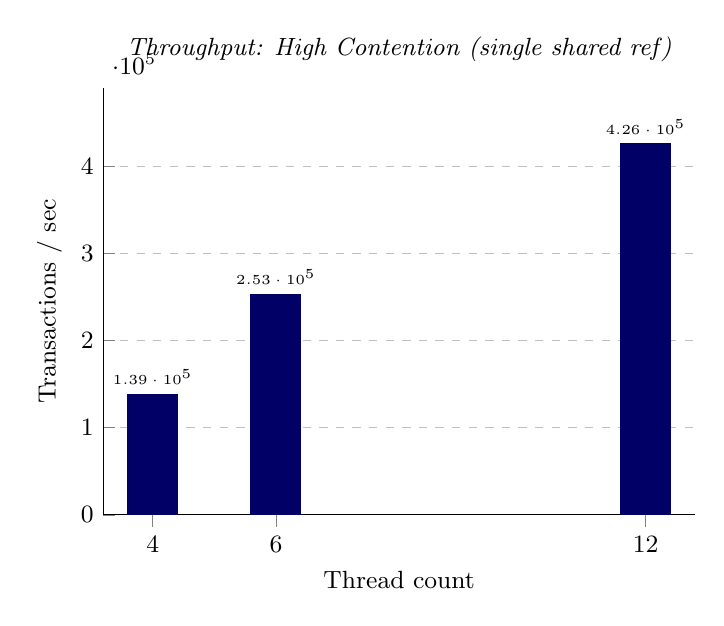
\begin{tikzpicture}
    \begin{axis}[
        title={Throughput: High Contention (single shared ref)},
        xlabel={Thread count}, ylabel={Transactions / sec},
        ybar, bar width=18pt, width=0.75\textwidth, height=7cm,
        xtick=data, ymin=0, enlarge y limits={upper, value=0.15},
        ymajorgrids=true, grid style=dashed,
        nodes near coords, nodes near coords align={vertical},
        every node near coord/.append style={font=\tiny, anchor=south},
        tick label style={font=\small}, label style={font=\small},
        title style={font=\small\itshape}, clip=false,
        axis y line*=left, axis x line*=bottom,
      ]
      \addplot[fill=blue!40!black, draw=blue!40!black] coordinates {
          (4,138633) (6,253421) (12,425973)
        };
    \end{axis}
  \end{tikzpicture}
  \caption{Throughput under maximal conflict. All threads write the same
    reference. Throughput scales from 139K to 426K\,TPS with zero commit-phase
    aborts at every thread count.}
  \label{fig:throughput-high-contention}
\end{figure}

\subsection{Low Contention}

Each thread works on its own private reference and never touches another
thread's data. There are no conflicts by construction, so every transaction
commits on its first attempt. This measures the baseline cost of the commit
path itself.

Throughput is 1,322,570\,TPS at 4 threads and falls to 1,092,815\,TPS at 6
threads and 1,033,984\,TPS at 12 threads. Even with no data conflicts, every
write transaction must acquire the global commit lock, so adding threads
creates a queue at that lock rather than useful parallelism. The JFR profiling
data in Section~\ref{sec:bottlenecks} confirms that all blocking in this
scenario is on that one lock.

\begin{figure}[H]
  \centering
  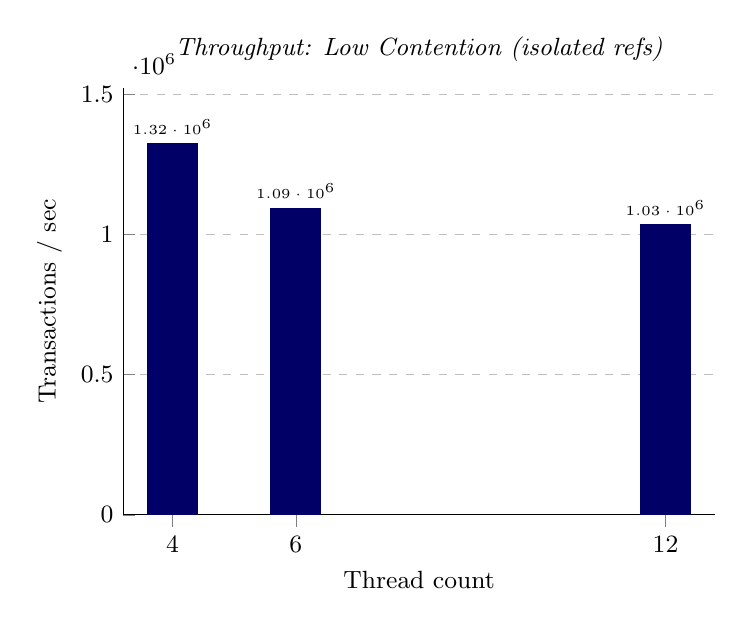
\begin{tikzpicture}
    \begin{axis}[
        title={Throughput: Low Contention (isolated refs)},
        xlabel={Thread count}, ylabel={Transactions / sec},
        ybar, bar width=18pt, width=0.75\textwidth, height=7cm,
        xtick=data, ymin=0, enlarge y limits={upper, value=0.15},
        ymajorgrids=true, grid style=dashed,
        nodes near coords, nodes near coords align={vertical},
        every node near coord/.append style={font=\tiny, anchor=south},
        tick label style={font=\small}, label style={font=\small},
        title style={font=\small\itshape}, clip=false,
        axis y line*=left, axis x line*=bottom,
      ]
      \addplot[fill=blue!40!black, draw=blue!40!black] coordinates {
          (4,1322570) (6,1092815) (12,1033984)
        };
    \end{axis}
  \end{tikzpicture}
  \caption{Throughput when each thread works on its own isolated reference.
    The declining profile reflects commit-lock queuing even under zero data
    contention.}
  \label{fig:throughput-low-contention}
\end{figure}

\subsection{Bank Transfer}

Threads randomly pick pairs of accounts from a shared pool of 20 and transfer
a random amount, committing only when the source account has sufficient funds.
Contention arises naturally since accounts are shared across all threads.

Throughput peaks at 213,631\,TPS at 4 threads and drops to 163,402\,TPS at
6 threads, recovering slightly to 173,725\,TPS at 12 threads. The decline
follows the same pattern as the low-contention scenario: nearly every
transaction writes to two accounts and must acquire the global commit lock,
which becomes the bottleneck as thread count grows.

Correctness is verified after each run by checking that the total balance
across all accounts equals the starting sum, which holds in every measurement.

\begin{figure}[H]
  \centering
  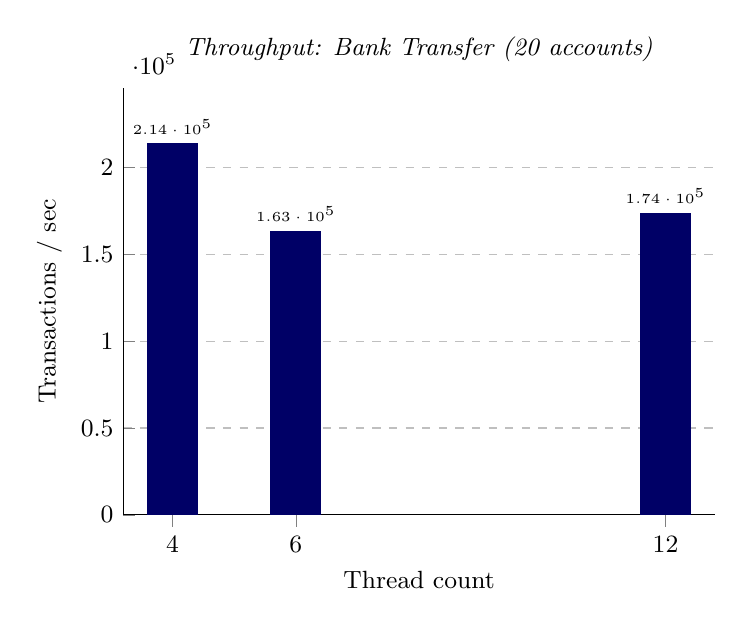
\begin{tikzpicture}
    \begin{axis}[
        title={Throughput: Bank Transfer (20 accounts)},
        xlabel={Thread count}, ylabel={Transactions / sec},
        ybar, bar width=18pt, width=0.75\textwidth, height=7cm,
        xtick=data, ymin=0, enlarge y limits={upper, value=0.15},
        ymajorgrids=true, grid style=dashed,
        nodes near coords, nodes near coords align={vertical},
        every node near coord/.append style={font=\tiny, anchor=south},
        tick label style={font=\small}, label style={font=\small},
        title style={font=\small\itshape}, clip=false,
        axis y line*=left, axis x line*=bottom,
      ]
      \addplot[fill=blue!40!black, draw=blue!40!black] coordinates {
          (4,213631) (6,163402) (12,173725)
        };
    \end{axis}
  \end{tikzpicture}
  \caption{Throughput under a realistic mixed workload with 20 shared
    accounts. Throughput peaks at 4 threads and declines at higher counts,
    consistent with the global commit lock being the bottleneck.}
  \label{fig:throughput-bank-transfer}
\end{figure}

\subsection{Read-Heavy and Write-Heavy Workloads}
\label{sec:read-write-heavy}

Both scenarios use a mixed workload over 10 shared references.

\paragraph{Read-Heavy (10\% writes).}
Each transaction either writes a randomly chosen reference (10\% probability)
or reads and sums all 10 references (90\% probability). Read-only transactions
skip the commit lock entirely, reading a consistent snapshot directly from the
version history.

This is the key advantage of the MVCC design. Throughput scales from
533,885\,TPS at 4 threads to 1,082,057\,TPS at 6 threads ($2.03\times$) and
1,969,463\,TPS at 12 threads ($3.69\times$): the strongest scaling result
in the suite and the clearest demonstration of the MVCC benefit.

\paragraph{Write-Heavy (90\% writes).}
With 90\% of transactions writing, nearly every transaction must acquire the
commit lock. Throughput falls monotonically: 637,709\,TPS at 4 threads,
418,108\,TPS at 6 threads ($0.66\times$), and 257,574\,TPS at 12 threads
($0.40\times$). Abort rates are zero throughout, ruling out retries as a
factor. The bottleneck is entirely the commit lock, confirmed by the JFR data
in Section~\ref{sec:bottlenecks}.

\begin{figure}[H]
  \centering
  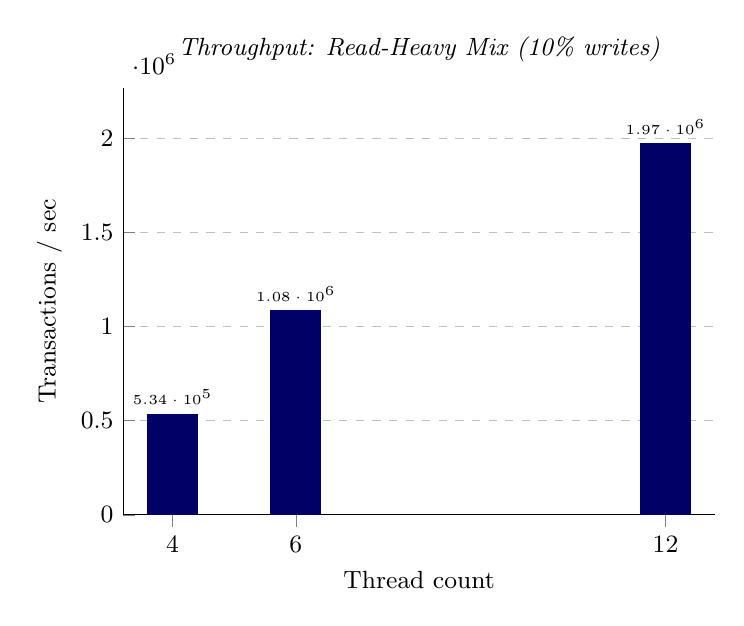
\begin{tikzpicture}
    \begin{axis}[
        title={Throughput: Read-Heavy Mix (10\% writes)},
        xlabel={Thread count}, ylabel={Transactions / sec},
        ybar, bar width=18pt, width=0.75\textwidth, height=7cm,
        xtick=data, ymin=0, enlarge y limits={upper, value=0.15},
        ymajorgrids=true, grid style=dashed,
        nodes near coords, nodes near coords align={vertical},
        every node near coord/.append style={font=\tiny, anchor=south},
        tick label style={font=\small}, label style={font=\small},
        title style={font=\small\itshape}, clip=false,
        axis y line*=left, axis x line*=bottom,
      ]
      \addplot[fill=blue!40!black, draw=blue!40!black] coordinates {
          (4,533885) (6,1082057) (12,1969463)
        };
    \end{axis}
  \end{tikzpicture}
  \caption{Throughput with 90\% read-only transactions. Readers access
    consistent snapshots without the commit lock, so additional threads
    contribute genuine parallelism. Throughput scales to 1.97M\,TPS at
    12 threads.}
  \label{fig:throughput-read-heavy}
\end{figure}

\begin{figure}[H]
  \centering
  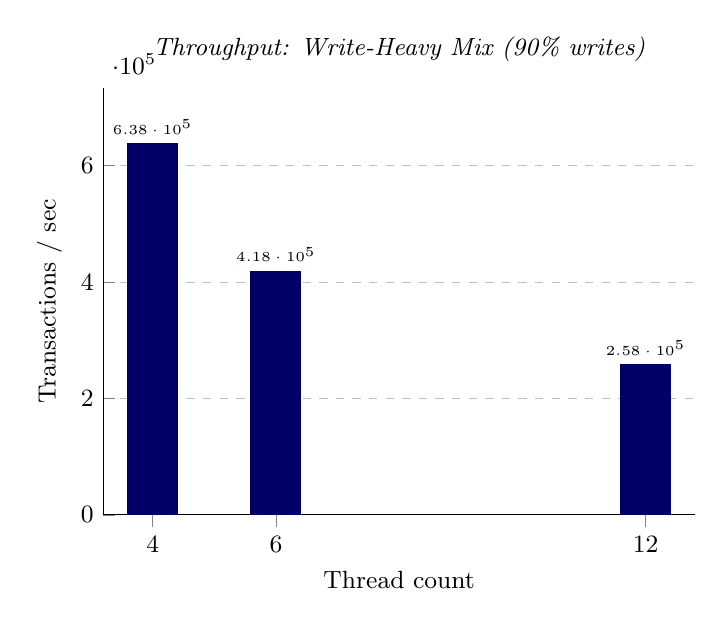
\begin{tikzpicture}
    \begin{axis}[
        title={Throughput: Write-Heavy Mix (90\% writes)},
        xlabel={Thread count}, ylabel={Transactions / sec},
        ybar, bar width=18pt, width=0.75\textwidth, height=7cm,
        xtick=data, ymin=0, enlarge y limits={upper, value=0.15},
        ymajorgrids=true, grid style=dashed,
        nodes near coords, nodes near coords align={vertical},
        every node near coord/.append style={font=\tiny, anchor=south},
        tick label style={font=\small}, label style={font=\small},
        title style={font=\small\itshape}, clip=false,
        axis y line*=left, axis x line*=bottom,
      ]
      \addplot[fill=blue!40!black, draw=blue!40!black] coordinates {
          (4,637709) (6,418108) (12,257574)
        };
    \end{axis}
  \end{tikzpicture}
  \caption{Throughput when 90\% of transactions write. The monotonically
    declining profile, combined with zero abort rates, confirms the commit
    lock as the sole bottleneck.}
  \label{fig:throughput-write-heavy}
\end{figure}

\section{Version History Size}
\label{sec:history-sweep}

Each reference keeps a short history of past values so that concurrent readers
can always find a consistent snapshot. A history that is too short causes reads
to fail when no valid snapshot exists (a \emph{trim abort}); one that is too
long increases read latency and generates more short-lived allocations per
commit, increasing garbage collection overhead. To characterize this
trade-off, the bank transfer scenario was repeated across history sizes of 8,
16, 32, 64, 128, and 256 at thread counts of 4, 6, and 12, with 50,000
transactions per thread.

\begin{table}[H]
  \centering
  \caption{Version history size sweep: bank transfer throughput and abort
    rates (20 accounts, 50{,}000 transactions per thread).}
  \label{tab:history-sweep}
  \begin{tabular}{@{}r r r r r@{}}
    \toprule
    \textbf{\texttt{max-history}}   & \textbf{Threads}            & \textbf{TPS} &
    \textbf{Conflict aborts/commit} & \textbf{Trim aborts/commit}                              \\
    \midrule
    8                               & 4                           & 405,530      & 0.17 & 0.00 \\
    8                               & 6                           & 518,980      & 0.15 & 0.00 \\
    8                               & 12                          & 328,653      & 0.33 & 0.00 \\
    \midrule
    16                              & 4                           & 532,988      & 0.15 & 0.00 \\
    16                              & 6                           & 475,417      & 0.15 & 0.00 \\
    16                              & 12                          & 276,301      & 0.41 & 0.00 \\
    \midrule
    32                              & 4                           & 505,626      & 0.10 & 0.00 \\
    32                              & 6                           & 526,794      & 0.14 & 0.00 \\
    32                              & 12                          & 318,387      & 0.34 & 0.00 \\
    \midrule
    64                              & 4                           & 518,794      & 0.13 & 0.00 \\
    64                              & 6                           & 454,909      & 0.18 & 0.00 \\
    64                              & 12                          & 322,807      & 0.33 & 0.00 \\
    \midrule
    128                             & 4                           & 515,565      & 0.13 & 0.00 \\
    128                             & 6                           & 520,253      & 0.15 & 0.00 \\
    128                             & 12                          & 250,567      & 0.48 & 0.00 \\
    \midrule
    256                             & 4                           & 494,023      & 0.13 & 0.00 \\
    256                             & 6                           & 502,525      & 0.12 & 0.00 \\
    256                             & 12                          & 226,295      & 0.49 & 0.00 \\
    \bottomrule
  \end{tabular}
\end{table}

Three results stand out.

First, trim aborts are zero across all history sizes and thread counts. The
bank transfer workload distributes writes across 20 accounts, so any single
reference is written infrequently relative to how fast history slots cycle. A
transaction's read point is always recent enough that \texttt{find-entry}
locates a valid snapshot. Trim aborts would appear in workloads that
concentrate writes on very few references, where a single ref could accumulate
enough commits to exhaust the history window before a concurrent reader
accesses it.

Second, history size has no consistent effect on throughput at 4 and 6 threads
across the range 8-256.

Third, at 12 threads throughput drops at sizes 128 and 256, falling from the
318,000-328,000\,TPS range seen at sizes 8-64 to 250,567 and 226,295\,TPS.
This is the only consistent directional effect in the table. The cause is
that \texttt{apply-writes!} appends a new entry to the history vector on every
commit via \texttt{conj}, and at sizes 128 and 256 these vectors are large
enough that the resulting allocation and GC cost becomes visible at 12 threads. 
At 4 and 6 threads the commit rate is lower and the overhead is not significant.

Conflict abort rates at 12 threads are elevated throughout (0.33-0.49),
consistent with the commit-lock pressure described in
Section~\ref{sec:bottlenecks}, but show no reliable correlation with history
size.

\begin{figure}[H]
  \centering
  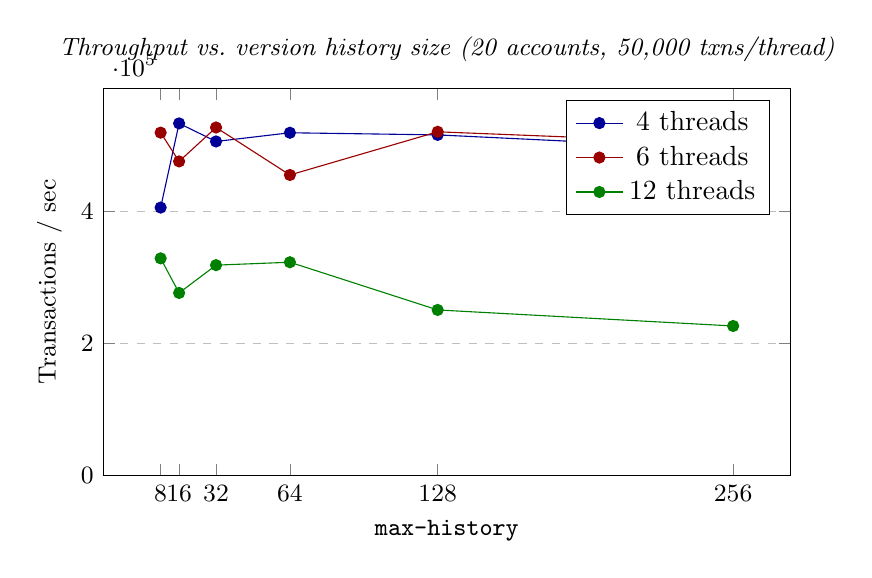
\begin{tikzpicture}
    \begin{axis}[
        title={Throughput vs.\ version history size (20 accounts,
            50{,}000 txns/thread)},
        xlabel={\texttt{max-history}},
        ylabel={Transactions / sec},
        width=0.85\textwidth, height=6.5cm,
        xtick={8,16,32,64,128,256},
        ymin=0,
        ymajorgrids=true, grid style=dashed,
        mark=*, tick label style={font=\small},
        label style={font=\small}, title style={font=\small\itshape},
        legend pos=north east,
      ]
      \addplot[color=blue!60!black, mark=*] coordinates {
          (8,405530) (16,532988) (32,505626) (64,518794) (128,515565) (256,494023)
        };
      \addlegendentry{4 threads}
      \addplot[color=red!60!black, mark=*] coordinates {
          (8,518980) (16,475417) (32,526794) (64,454909) (128,520253) (256,502525)
        };
      \addlegendentry{6 threads}
      \addplot[color=green!50!black, mark=*] coordinates {
          (8,328653) (16,276301) (32,318387) (64,322807) (128,250567) (256,226295)
        };
      \addlegendentry{12 threads}
    \end{axis}
  \end{tikzpicture}
  \caption{Throughput across version history sizes at 50,000 transactions per
    thread. At 4 and 6 threads throughput is flat across all sizes. At 12
    threads it declines at sizes 128 and 256 due to GC overhead from large
    history vectors. Trim aborts are zero throughout.}
  \label{fig:history-sweep}
\end{figure}

\section{Latency Analysis}

Figure~\ref{fig:bank-contention-latency} shows mean transaction latency across
four scenarios on a logarithmic scale. The logarithmic axis is necessary
because the extreme-contention case is roughly two orders of magnitude slower
than the no-contention baseline.

\paragraph{Scenario (i): single uncontended transfer.}
A single transfer between two fixed accounts with no concurrent threads. This
is the baseline cost of a complete commit: reading the current value, preparing
the write, acquiring the lock, validating reads, applying the write, and
dispatching any registered callbacks. Baseline latency is
\textbf{1.76\,$\mu$s} ($\pm$\,0.03).

\paragraph{Scenario (ii): extreme contention.}
Multiple concurrent threads all target the same two accounts simultaneously.
Latency rises to \textbf{401.56\,$\mu$s} ($\pm$\,35.25), a $228\times$
increase. The large standard deviation (about 9\% of the mean) reflects how
long a thread has to wait before retrying after a conflict.

\paragraph{Scenarios (iii) and (iv): callback overhead.}
These scenarios measure the cost of \texttt{on-commit} callbacks,
single-threaded with no concurrency. Scenario~(iii) is the no-callback
baseline at \textbf{1.59\,$\mu$s} ($\pm$\,0.03); scenario~(iv) adds a
callback at \textbf{1.81\,$\mu$s} ($\pm$\,0.08). The difference,
\textbf{0.22\,$\mu$s}, is the cost of dispatching the callback, roughly
14\% of the baseline commit cost. The small difference between scenarios~(i)
and~(iii) (1.76 vs.\ 1.59\,$\mu$s) is within normal measurement variation
between separate Criterium runs.

\begin{figure}[htbp]
  \centering
  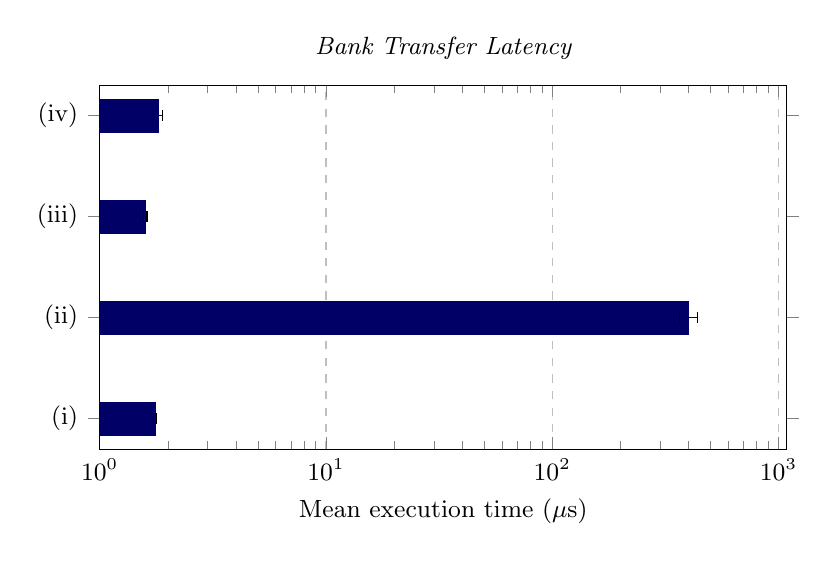
\begin{tikzpicture}
    \begin{axis}[
        title={Bank Transfer Latency},
        xlabel={Mean execution time ($\mu$s)},
        width=0.85\textwidth, height=6.2cm,
        xbar, bar width=12pt, xmode=log, xmin=1,
        enlarge x limits={upper, value=0.15},
        ytick={0,1,2,3},
        yticklabels={(\romannumeral 1),(\romannumeral 2),(\romannumeral 3),(\romannumeral 4)},
        xmajorgrids=true, grid style=dashed,
        tick label style={font=\small}, label style={font=\small},
        title style={font=\small\itshape},
      ]
      \addplot[fill=blue!40!black, draw=blue!40!black,
        error bars/.cd, x dir=both, x explicit
      ] coordinates {
          (1.758,0) +- (0.030,0)
          (401.556,1) +- (35.249,0)
          (1.587,2) +- (0.032,0)
          (1.810,3) +- (0.077,0)
        };
    \end{axis}
  \end{tikzpicture}
  \vspace{0.5em}
  \begin{minipage}{0.85\textwidth}
    \centering \small
    \begin{tabular}{@{}r l@{}}
      (\romannumeral 1) & single transfer, no concurrency                   \\
      (\romannumeral 2) & same transfer under extreme concurrent load       \\
      (\romannumeral 3) & single transfer, no callback registered           \\
      (\romannumeral 4) & single transfer, with \texttt{on-commit} callback \\
    \end{tabular}
  \end{minipage}
  \caption{Bank transfer latency on a logarithmic axis. Scenarios~(i) and
    (iii)--(iv) are single-threaded; scenario~(ii) uses concurrent threads
    all targeting the same two accounts.}
  \label{fig:bank-contention-latency}
\end{figure}

\section{Discussion}

\subsection{Architectural Strengths}

The results confirm two clear strengths of the design.

The first is the MVCC read path. Read-only transactions never acquire any
lock, they read a consistent snapshot directly from the version history.
This is why the read-heavy scenario scales to 1,969,463\,TPS at 12 threads
($3.69\times$ from 4 threads), outperforming every other scenario at high
thread counts and being the only scenario in the suite to scale beyond the
physical core count.

The second is the low overhead of \texttt{on-commit} callbacks: 0.22\,$\mu$s,
or roughly 14\% of the single-threaded baseline. Side-effect coordination can
be added to the transactional model without meaningful overhead.

Abort rates are zero across all throughput scenarios. Even under maximum
contention, conflicts are caught at write time by the ownership protocol, so
no transaction ever reaches commit and fails there.

\subsection{Identified Bottleneck: the Commit Lock}
\label{sec:bottlenecks}

The dominant bottleneck across all write-heavy scenarios is the \textbf{global
  commit lock}. Every write transaction must acquire it to record its result.
When multiple threads compete for it, they queue and wait, directly reducing
throughput.

The JFR profiling data makes this concrete. In the write-heavy scenario, a
single lock accounts for all thread blocking in the process.
Table~\ref{tab:jfr-summary} shows total time threads spent waiting for that
lock at each thread count.

\begin{table}[H]
  \centering
  \caption{JFR commit-lock profiling: write-heavy scenario. All blocking is
    concentrated on a single lock. The 12-thread run shows a second lock with
    one brief event, accounting for 3\% of total blocked time.}
  \label{tab:jfr-summary}
  \begin{tabular}{@{}r r r r r@{}}
    \toprule
    \textbf{Threads}              &
    \textbf{Total wait (B ticks)} &
    \textbf{Avg wait (M ticks)}   &
    \textbf{Max wait (M ticks)}   &
    \textbf{Lock events}                                  \\
    \midrule
    4                             & 1.54 & 110 & 163 & 14 \\
    6                             & 2.81 & 134 & 183 & 21 \\
    12                            & 5.55 & 121 & 186 & 46 \\
    \bottomrule
  \end{tabular}
\end{table}

Two observations follow.

First, total wait time grows faster than thread count. Going from 4 to 12
threads ($3\times$ more workers) causes total wait time to grow $3.6\times$,
from 1.54\,B to 5.55\,B ticks. This is the signature of a saturated lock:
each new thread makes every other thread wait longer.

Second, the maximum wait per event is stable across thread counts
(163-186\,M ticks). Individual commits are not slower at higher concurrency;
threads simply queue for longer. This means replacing the single global lock
with per-reference or per-stripe locks would recover the lost throughput
without changing how commits work internally.

This directly motivates the per-stripe commit lock discussed in
Section~\ref{sec:future}.
\chapter{Conclusion}

\section{Summary}

This work set out to build a Software Transactional Memory system in Clojure
that closes a specific gap in the existing ecosystem: there was no safe way
to coordinate side-effects such as logging or notifications at transaction
boundaries. What came out of it is an STM implementation based on a variation
of TL2, extended with MVCC and a transactional event system, together with a
formal proof that every history the system produces satisfies
opacity~\cite{guerraoui2007}.

The evaluation results were not uniform, but they were informative.
Read-heavy workloads scale well, reaching 1.97M\,TPS at 12 threads, since
read-only transactions skip the commit lock entirely and run in genuine
parallel. High-contention workloads scale too, for a different reason: the
ownership protocol catches conflicts eagerly at write time rather than
waiting until commit. Write-heavy workloads are the exception: the global
commit lock serialises every write commit, so past the saturation point,
adding threads actively hurts throughput rather than helping it. As for the
transactional event system itself, it adds 0.22\,$\mu$s per commit, roughly
14\% over baseline, which is a small price given what it buys.

\section{Limitations and Future Work}
\label{sec:future}

\paragraph{Global commit lock.}
The most pressing limitation is the global commit lock. Section~\ref{sec:bottlenecks}
shows it accounts for nearly all thread blocking in write-heavy scenarios,
with total wait time growing faster than thread count once the lock
saturates. One fix stands out: replace the single lock with a fixed array of
per-stripe locks, hashing each reference to a stripe, following TL2's PS
policy~\cite{dice2006transactional}. Two write transactions landing on
different stripes could then commit in parallel, recovering the throughput
currently lost to serialisation without touching how an individual commit
works internally.

\paragraph{Dynamic version history sizing.}
The history-sweep results in Section~\ref{sec:history-sweep} show a fixed
global bound working well enough for the bank transfer workload, since trim
aborts never occur there, but nothing guarantees that holds more generally.
A workload combining short, frequent writes on a small number of references
with long-running read transactions could exhaust the history window before
a reader gets a chance to use it, producing trim aborts that a larger history
would have avoided. Simply raising \texttt{max-history} runs into the GC
overhead already visible at 12 threads for sizes 128 and 256. Clojure's own
STM avoids this trade-off by letting each reference track its own abort rate
and grow its history independently once trim aborts start occurring.
Something similar here would remove the need to hand-tune
\texttt{max-history}, and would likely cut abort rates in the workloads
where a fixed bound currently struggles.

\paragraph{Lifecycle hook granularity.}
The current hook model offers two attachment points, \texttt{on-commit} and
\texttt{on-rollback}, which covers most use cases but not all of them. A
\texttt{before-commit} hook, firing after read-set validation but before
writes are applied, would open the door to write-ahead logging: the pending
write set could be appended to a persistent log while the transaction still
holds the commit lock, giving durability guarantees the current model has no
way to express. Further phases such as \texttt{after-commit},
\texttt{before-retry}, and \texttt{after-retry} would extend this further,
covering use cases that need to act at specific points in the lifecycle
rather than only at its terminal boundaries.

\bibliographystyle{abbrvnat}
\bibliography{references}

\end{document}